\documentclass{article}

\usepackage{amsmath}
\usepackage{textcomp}
\usepackage[a4paper, total={6in, 8in}]{geometry}
\usepackage{graphicx}
\usepackage{caption}
\usepackage{subcaption}
\usepackage{amssymb}
\usepackage{listings}
\usepackage{color} %red, green, blue, yellow, cyan, magenta, black, white
\definecolor{mygreen}{RGB}{28,172,0} % color values Red, Green, Blue
\definecolor{mylilas}{RGB}{170,55,241}


\begin{document}

\begin{titlepage}
	\centering
	{\scshape\LARGE \v{C}VUT FSv  \par}
	\vspace{1cm}
	{\scshape\Large 101MA02 Semester Project\par}
	\vspace{1.5cm}
	{\huge\bfseries Earthquake's effect on a multistory building: a simple model\par}
	\vspace{2cm}
	{\Large\textbf{Kalin Ivanov}\par}
	\vspace{2cm}
	{\large \today\par}
	\vfill
	%{\small supervised by\par}
	%\vspace{1cm}
	{\Large supervised by Ing. Michal Bene\v{s}, Ph.D\par}
	

% Bottom of the page
	
\end{titlepage}

%	\maketitle
	\pagenumbering{gobble}

	\newpage
	\tableofcontents
	\pagenumbering{gobble}
	
	\newpage
	\pagenumbering{arabic}

%%%%%%%%%%%%%%%%%%%%%%%%%%%%%%%%%%%%%%%%%%%%%%%%%%%%%%%% INTRO
%%%%%%%%%%%%%%%%%%%%%%%%%%%%%%%%%%%%%%%%%%%%%%%%%%%%%%%%%%%
	
	\section{Abstract}

Earthquakes are major disasters that cause great amounts of damage to buildings as they put into motion structures not meant to move. There are several factors that determine building resistance to motion including, mass, number of floors, influence of damping and material properties. These parameters are explored and analyzed in a simple model that approximates a multistory building, or any structure that is composed of multiple elastically connected, inertial sections. It is imperative that the effects of earthquakes on structures are well understood and modelled to design buildings effectively and safely. The purpose of this paper is to explore the different mathematical techniques used to solve the equations associated with the motion of multi-story buildings. 

	\section{Model description}

		 	\paragraph{The building} A great simplification of a multistory building will allow for a relatively simple, yet effective model to examine the effect of an earthquake's shaking on the building's structure. Each floor can be thought of as a point mass that is connected to the floor above it and below it through rigid beams that are connected by springs (See Figure \ref{fig1}). The assumption is that the connections between the floors will behave elastically to the force caused by the earthquake. It is important to note, that the model attempts to explain only the horizontal displacements caused by the earthquake.
				
				\begin{figure}[h!]
   					\centering
   					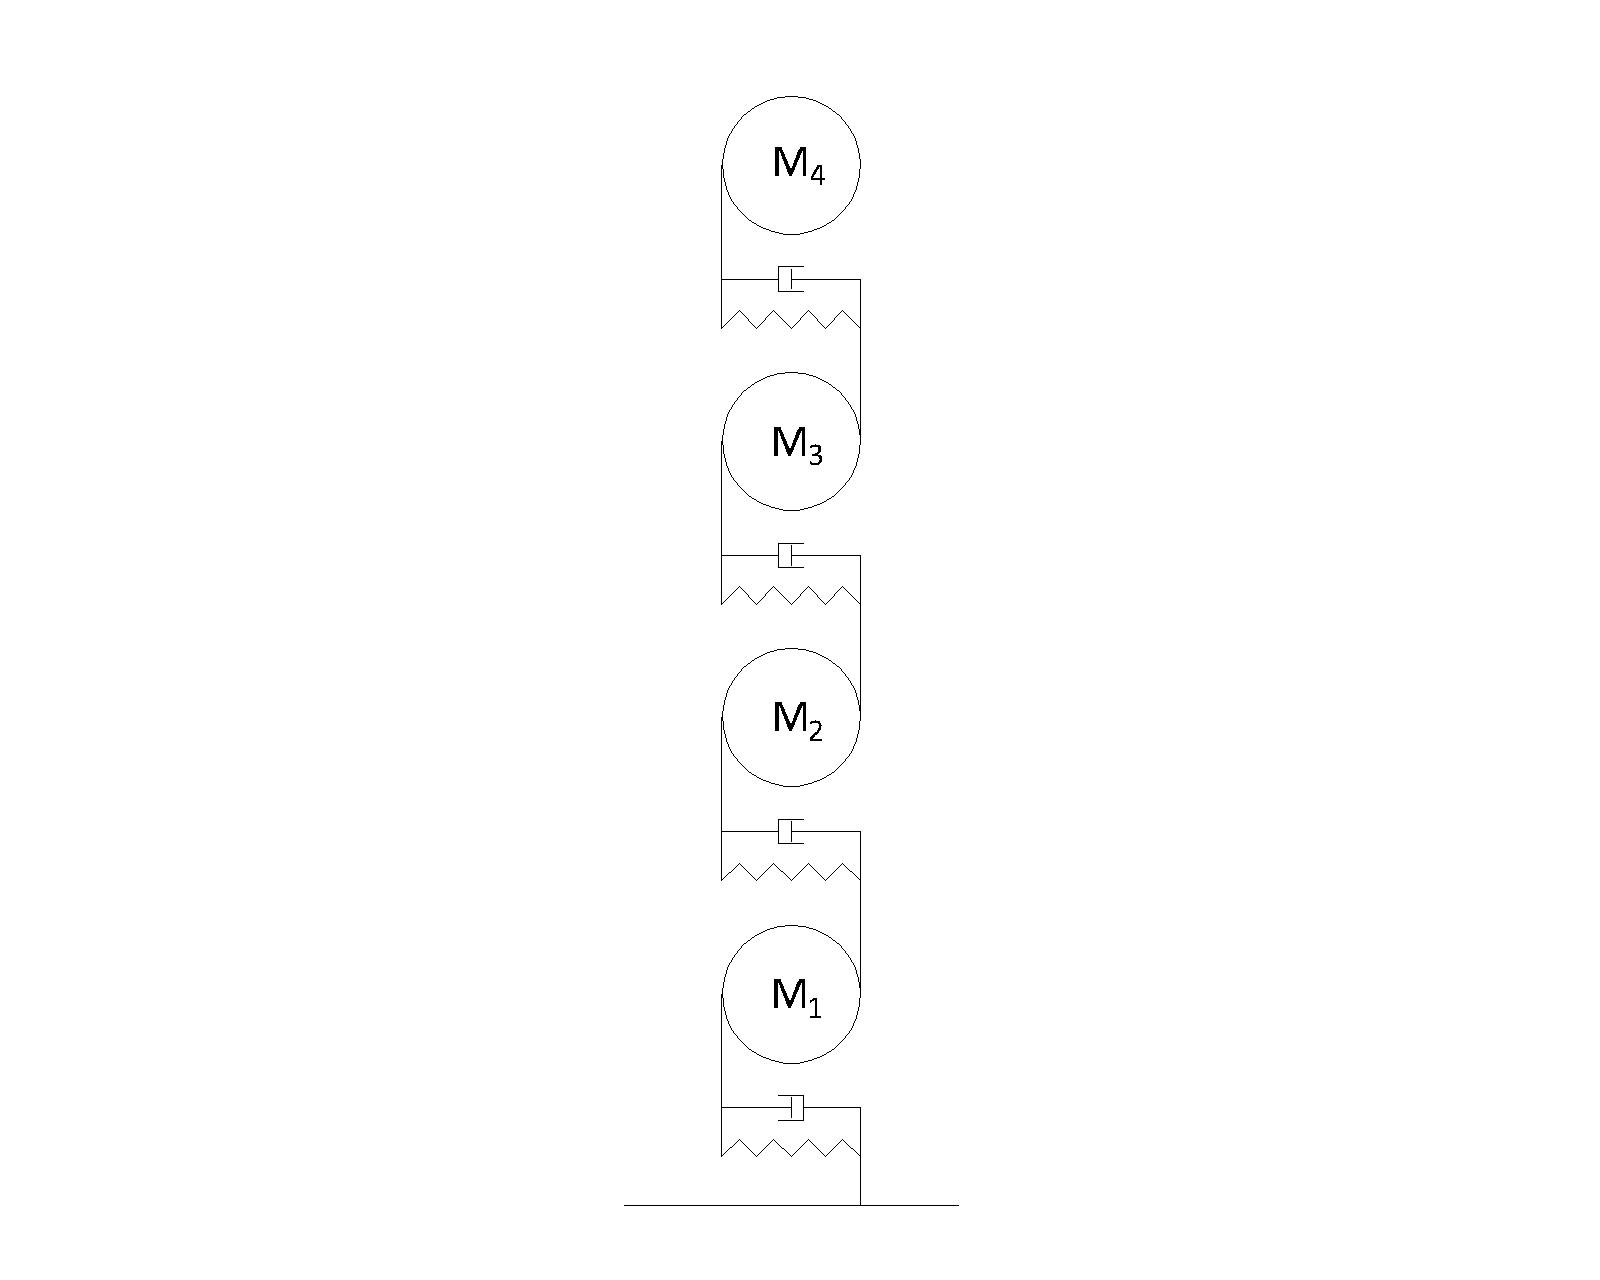
\includegraphics[width=120mm]{SPRINGS-Model1.jpg}
					\centering
   					\caption{4-story point-mass building model}
					\medskip
					\small
					Each floor is represented by a point mass connected with the other floors by springs and dashpots.
				           \label{fig1}
  				\end{figure}

			\paragraph{Assumptions} Although models that approximate earthquake movement exist, we will mostly be concerned with the modelling of the building's motion rather than the motion of the ground caused by the earthquake. The motion introduced by the earthquake can be regarded as a simple periodic force (cosine function) for our purposes. The displacement of each floor will be based on the displacements of the floors it is attached to. Before the earthquake begins, the ground is at initial position $x_0 = 0$ and each $i^{th}$ floor has an initial position $x_i(0)$ (that coincides with the initial position of the ground if it is a straight building, see Figure \ref{fig2}). As the earthquake begins each floor will be displaced relative to the ground given by $x_i(t)$. As the ground moves side to side, each floor’s spring will respond with a force in the opposite direction to the spring force of the floor below and above it, by Newton’s Third Law. A damping force will also be considered in the same manner as the elastic force. 
				
				\begin{figure}[h!]
  					\centering
 				 	\begin{minipage}[b]{0.4\textwidth}
    						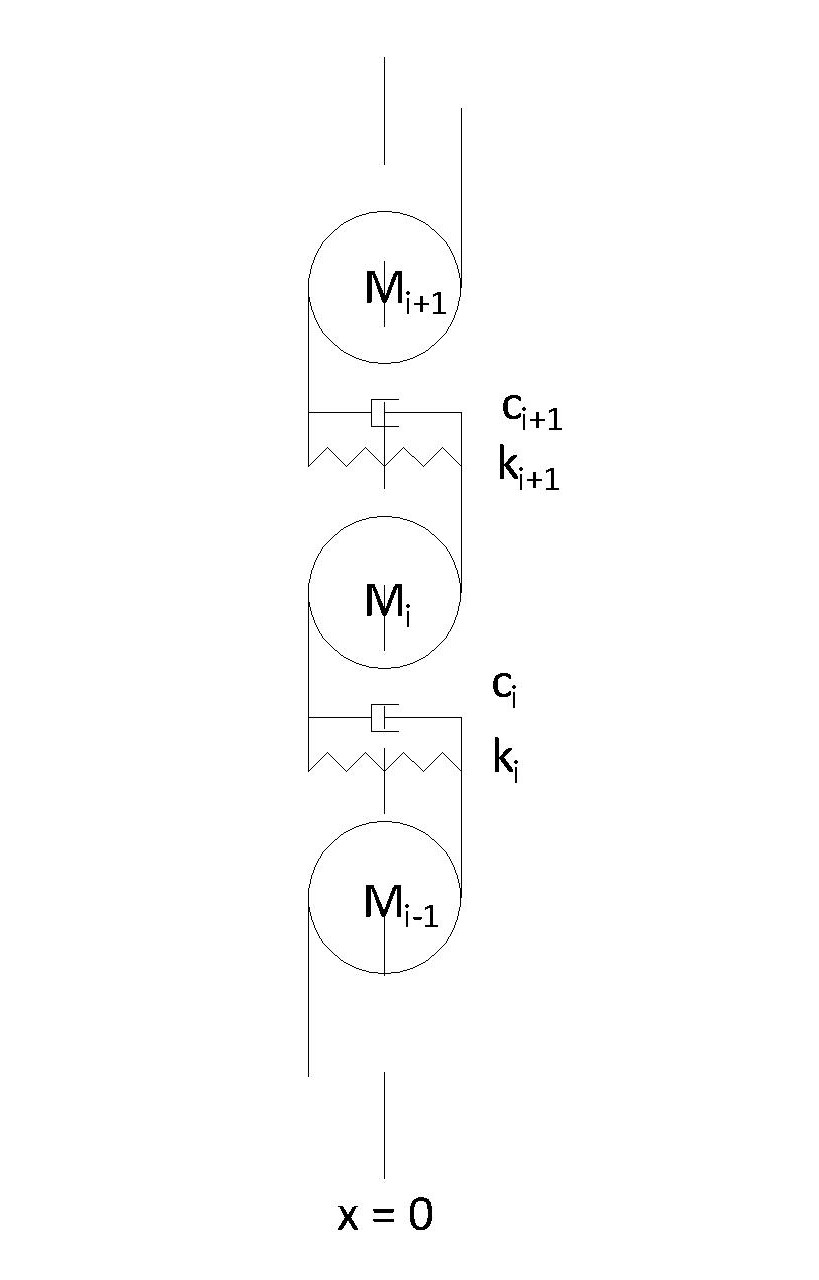
\includegraphics[width=65mm]{SPRINGS-Model2A.jpg}
    						\caption{$i^{th}$ floor statics}
						\medskip
						\small
						$M_i$ is the mass of the $i^{th}$ floor, $c_i$ is the damping constant between the $i^{th}$ and the $(i-1)^{th}$ floors, $k_i$ is the spring constant between the $i^{th}$ and the $(i-1)^{th}$ floors. Similarly $c_{i+1}$ and $k_{i+1}$ are the corresponding costants between the $i^{th}$ and the $(i+1)^{th}$ floors.
						\label{fig2}
  					\end{minipage}
 					 \hfill
					\begin{minipage}[b]{0.4\textwidth}
 				  	 	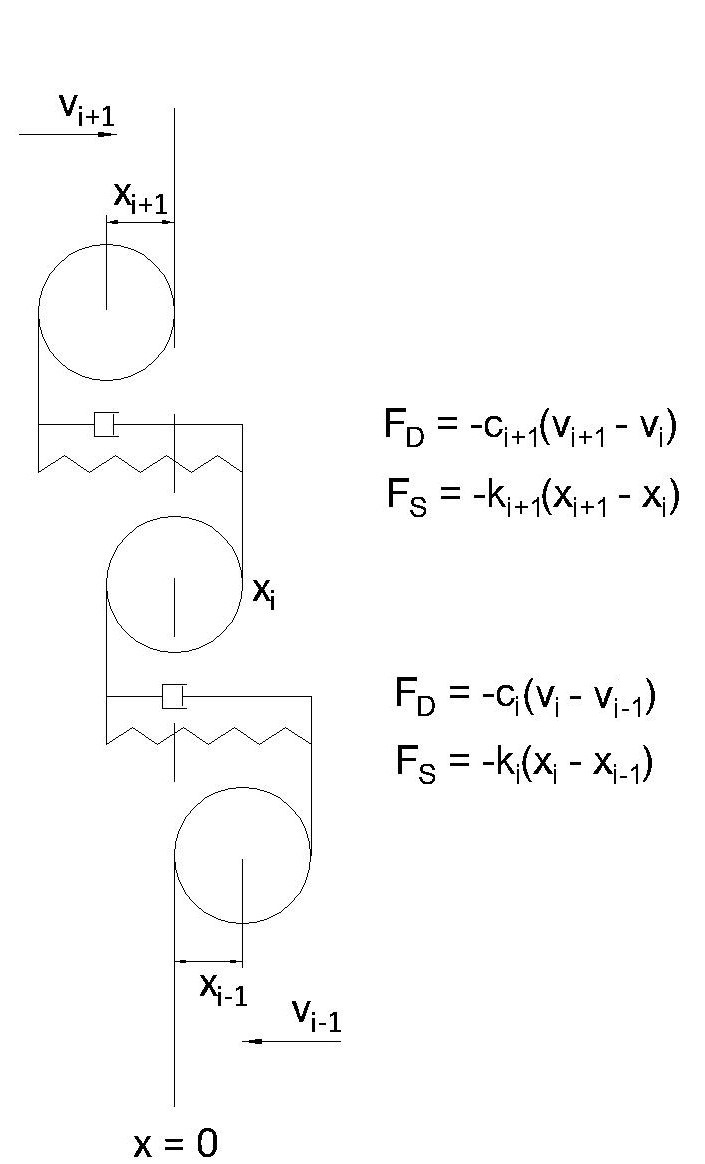
\includegraphics[width=60mm]{SPRINGS-Model3A.jpg}
    						\caption{$i^{th}$ floor dynamics}
						\medskip
					\small
					$x_i$ is the position of the $i^{th}$ floor relative to the center of mass reference frame $x = 0$. $F_D$ is the damping force which is proportional via $c$ to the difference in velocity between 2 floors. $F_S$ is the spring force, proportional via $k$ to the difference in position between 2 floors. 
						\label{fig3}
 					 \end{minipage}
				\end{figure}

			\paragraph{Motion} As a floor moves from its initial position, a spring and damping force will be induced. We make the following assumptions regarding the motion of the building. The spring force will act linearly, that is, as the floor moves farther and farther away from its initial position, a greater and greater force (increasing linearly) will be acting on the floor to restore it back to the original position. This is Hooke's Law given by $m\frac{d^2x}{dt^2} = - kx$, where $m$ is the mass, $k$ is the spring constant, $x$ is the displacement, $\frac{d^2x}{dt^2}$ is the acceleration. Considering just the damping force in a similar manner, the force is  proportional to the velocity of the floor given by $m\frac{d^2x}{dt^2} = - c\frac{dx}{dt}$. When a floor is displaced, the forces acting on it will be the restoring and damping forces of the springs and dashpots on either side of the floor (see Figure \ref{fig3}) and that is why the signs of the force are negative (act opposite to the direction of motion). At a certain point the forces of the floor above and below acting on a given floor will be 0, which will be the point at which maximum displacement from the initial position is reached (this position is the amplitude of the oscillation). It is important to analyze the amplitude and frequency of oscillation of each floor to predict how the building will behave as an earthquake progresses. This will be analyzed in detail from now on. 

%%%%%%%%%%%%%%%%%%%%%%%%%%%%%%%%%%%%%%%%%%%%%%%%%%%% MATH DESCRIP

	\section{Mathematical description}

		\subsection{Notation} The notation of this paper differs between matrices, vectors and scalars in the following manner: Matrices are given in bold capital letters ($\textbf{M}$), vectors are in capital letters ($V$) and scalars are given in lowercase letters ($s$). The vectors $X$ , $V$ and $A$ represent position, velocity and acceleration, respectively. The vector $U$ is the vector of position and velocity: $U = \begin{bmatrix}X\\V\end{bmatrix}$.

		\subsection{System of differential equations}

			Dynamical equations can be written for each floor, which gives the following system of coupled ODEs
				
				\begin{align*}
					m_1\ddot{x}_1&= -k_1x_1 + k_2(x_2-x_1) - c_1\dot{x}_1 + c_2(\dot{x}_2-\dot{x}_1) + f_1\\
					m_2\ddot{x}_2&= -k_2(x_2-x_1) + k_3(x_3-x_2) -c_2(\dot{x}_2-\dot{x}_1) + c_3(\dot{x}_3-\dot{x}_2) + f_2\\
					&\vdots\\
					m_n\ddot{x}_n&= -k_n(x_n-x_{n-1}) - c_n(\dot{x}_n-\dot{x}_{n-1})+ f_n\\
				\end{align*}
Here for each $i$th floor $k_i$ is the elastic constant of the spring,  $c_i$ is the damping constant of the dashpot, $m_i$ is the mass of the floor, $x$, $\dot{x}$, and $\ddot{x}$ are the displacement, velocity and acceleration, respectively, and $n$ is the number of floors. The $f_i$ represents the forcing function present on each floor. We will consider $f_1 \neq 0$ and all other $f_i = 0$, since the forces generated by earthquakes only act on the first floor. Notice that all floors (except from the ground and last floors) have the same equation form: Hooke's law applied to the position change and damping applied to the velocity change regarding the $i$th, $(i-1)$th and $(i+1)$th floors. 

		\subsection{Matrix form}	

			For the general case of $n$-floors, we will make $n$ by $n$ matrices for the masses, elastic constants, and damping constants. This will allow for a compact equation form:

				\begin{equation}
					\textbf{M}\ddot{X}+\textbf{C}\dot{X}+\textbf{K}X = F
				\end{equation}
where \textbf{M} is the mass matrix, \textbf{C} is the damping matrix, \textbf{K} is the elastic matrix and $F$ is the vector representing the forcing function. In particular \textbf{M}, \textbf{C} and \textbf{K} take the form

				\begin{equation*}
					\textbf{M}=
					\begin{bmatrix}
						m_1 & 0 & 0 & \cdots & 0\\
						0 & m_2 & 0 & \cdots & 0\\
						\vdots & \vdots & \vdots & \ddots & \vdots \\
						0 & 0 & 0 & \cdots & m_n
					\end{bmatrix},\ \ 
				\end{equation*} \\

				\begin{equation*}
					\textbf{K}=
					\begin{bmatrix}
						k_1 + k_2 & -k_2 & 0 & 0 & \cdots & 0 & 0 & 0\\
						-k_2 & k_2 + k_3 & -k_3 & 0 & \cdots & 0 & 0 & 0\\
						0& -k_3 & k_3 + k_4 & -k_4 & \cdots & 0 & 0 & 0\\
						\vdots & \vdots & \vdots & \vdots & \ddots & \vdots & \vdots & \vdots \\
						0& 0 & 0 & 0 & \cdots & -k_{n-1} & k_{n-1}+k_{n} & -k_{n}\\
						0& 0 & 0 & 0 & \cdots & 0 & -k_{n} & k_{n}\\
					\end{bmatrix},\ \ 
				\end{equation*}\\

				\begin{equation*}
					\textbf{C}=
					\begin{bmatrix}
					           c_1 + c_2 & -c_2 & 0 & 0 & \cdots & 0 & 0 & 0\\
						-c_2 &  c_2 + c_3 & -c_3 & 0 & \cdots & 0 & 0 & 0\\
						0& -c_3 & c_3 + c_4 & -c_4 & \cdots & 0 & 0 & 0\\
						\vdots & \vdots & \vdots & \vdots & \ddots & \vdots & \vdots & \vdots \\
						0& 0 & 0 & 0 & \cdots & -c_{n-1} & c_{n-1}+c_{n} & -c_{n}\\
						0& 0 & 0 & 0 & \cdots & 0 &-c_{n-1} & c_{n}\\
					\end{bmatrix},\ \ 
				\end{equation*}\\
and
				\begin{equation*}
					F=
					\begin{bmatrix}
						f_1(t)\\
						0\\
						\vdots \\
						0
					\end{bmatrix}
					X=
					\begin{bmatrix}
						x_1(t)\\
						x_2(t)\\
						\vdots \\
						x_n(t)
					\end{bmatrix}
					\dot{X}=
					\begin{bmatrix}
						\dot{x}_1(t)\\
						\dot{x}_2(t)\\
						\vdots \\
						\dot{x}_n(t)
					\end{bmatrix}
					\ddot{X}=
					\begin{bmatrix}
						\ddot{x}_1(t)\\
						\ddot{x}_2(t)\\
						\vdots \\
						\ddot{x}_n(t)
					\end{bmatrix}
				\end{equation*}
\\
This representation of the problem is an initial value problem where the second order system of ODEs (1) is subject to some initial conditions $X(0)$, $V(0)$, which are the initial positions and velocities of each floor at time 0. 
				\paragraph{Solving the equation of motion} (1) is the equation of motion and solving it allows the analysis of the behavior of structures under the action of earthquakes. In some special cases relatively simple analytical solutions are possible, while in general it is more advantageous to use numerical approaches. Here are the cases:
\\
			
				\begin{enumerate}
  					\item Free motion - there is no forcing function, making the system homogeneous (this will be the first case considered).
  					\item Forced motion - there is a forcing function, making the system nonhomogeneous. Forced motion can be further distinguished into:
					\begin{itemize}
						\item Steady motion - An analytical description is possible
							\begin{enumerate}	
								\item Harmonic motion - Simplest case with sine and cosine functions
	 							\item Periodic motion - Fourier analysis possible
							\end{enumerate}
	 					\item Transient motion - Forces with impulses, that might not be continuous. Here numerical methods are needed.
					\end{itemize}
				\end{enumerate}

				\paragraph{Note} Here we will only consider linear elastic and damping behavior (that is the constants of elasticity and damping are constant). Nonlinear cases are examined in \cite{Hughes}.


%%%%%%%%%%%%%%%%%%%%%%%%%%%%%%%%%%%%%%%%%%%%%%%%%%%%% ANALYT SOL
%%%%%%%%%%%%%%%%%%%%%%%%%%%%%%%%%%%%%%%%%%%%%%%%%%%%%%%%%%%

	\section{Analytical solution}

		\subsection{Homogeneous system}

			To begin solving
				
				\begin{equation*}
					\textbf{M}\ddot{X}+\textbf{C}\dot{X}+\textbf{K}X = F
				\end{equation*}
let us first solve the homogenous equation

				\begin{equation}
					\ddot{X}+\textbf{G}\dot{X}+\textbf{Q}X = 0
				\end{equation}
where $\textbf{G} = \textbf{M}^{-1}\textbf{C}$ and $\textbf{Q} = \textbf{M}^{-1} \textbf{K}$ and afterwards find a particular solution for the nonhomogeneous equation. It will be convenient to reduce the order of this second order system to a first order system. Let $U_1 = X$, $U_2 = \dot{X}$ and $U = \begin{bmatrix} U_1 \\ U_2 \end{bmatrix}$. Then

				\begin{equation*}
					\ddot{X}=-\textbf{G}\dot{X}-\textbf{Q}X
				\end{equation*}
becomes

				\begin{align*}
					&\dot{U_1}=\dot{X}\\
					&\dot{U_2}=-\textbf{Q}X-\textbf{G}\dot{X}
				\end{align*}
or 

				\begin{equation}
					\dot{U}=\textbf{H}U
				\end{equation}
where 

				\begin{equation*}
					\dot{U}=\begin{bmatrix}\dot{X}\\ \ddot{X}\end{bmatrix}\text{,     } U=\begin{bmatrix}X\\ \dot{X}\end{bmatrix} \text{     and     } \\ \\  \textbf{H} = \begin{bmatrix} \textbf{0} & \textbf{I} \\ -\textbf{G} &-\textbf{Q} \end{bmatrix}.
				\end{equation*}\\
It is tempting to guess at a solution to (3) in the form $X = Be^{\lambda t}$, where $B$ is a vector of constants and $\lambda$ is any number. After substituting we get

				\begin{equation}
					B\lambda e^{\lambda t} = \textbf{H}Be^{\lambda t}
				\end{equation}
This becomes

				\begin{equation}
					 (\textbf{H} -\lambda\textbf{I})B= 0
				\end{equation}
To find a nontrivial solution $X$ we must find a nontrivial solution of (4), so

				\begin{equation}
					\text{det}(\textbf{H} - \lambda \textbf{I}) = 0
				\end{equation}
Now it is apparent that $\lambda$ is an eigenvalue and $B$ is the corresponding eigenvector of \textbf{H}. Because (6) will end up being the solution to a polynomial in $\lambda$, in general $\lambda$ can be any complex number in the form $\lambda = \alpha + i\beta$. Thus the solution of (2) is 

				\begin{equation}
					U = Be^{(\alpha + i\beta)t}
				\end{equation}
However, if the eigenvalue $\lambda$ is complex so is the eigenvector $B = \text{Re}(B) + i\text{Im}(B) $. Using Euler's formula the solution can be written as 

				\begin{equation*}
					U = [\text{Re}(B) + i\text{Im}(B)]e^{\alpha t}(\cos{\beta t}+ i\sin{\beta t})
				\end{equation*}
Observing that if $y + iz$ is a solution to (3) and substituting

				\begin{equation*}
					\dot{y} + i\dot{z} = \textbf{H}y + \textbf{H}iz
				\end{equation*}
we see that $y$ and $z$ are both real solutions of (3). Thus, 2 real, linearly independent solutions are 

				\begin{align}
					&U_1 = e^{\alpha t}\left[\text{Re}(B)\cos{\beta t} -\text{Im}(B)\sin{\beta t}\right]\\
					&U_2 = e^{\alpha t}\left[\text{Im}(B)\cos{\beta t} +\text{Re}(B)\sin{\beta t} \right]
				\end{align}
and by the superposition principle the general solution of (3) is

				\begin{equation*}
					U = \textbf{C}_1U_1 + \textbf{C}_2U_2
				\end{equation*}
where $\textbf{C}_1$ and $\textbf{C}_2$ are diagonal matrices of arbitrary constants.
			\paragraph{Note} Complex eigenvalues always come in conjugate pairs $\lambda = \alpha + i\beta$ and $\bar{\lambda}= \alpha - i\beta$ with conjugate pair eigenvectors $B$ and $\bar{B}$. However, since the only difference in solution will be the sign on the sine term in (8) and (9), the effects of the conjugate pair will be masked in the constant vectors in the general solution. This means we need to consider only 1 complex eigenvalue of the conjugate pair for the general solution. As demonstrated above 1 complex eigenvalue will produce 2 linearly independent real solutions.

%%%%%%%%%%%%%%%%%%%%%%%%%%%%%%%%%%%%%%%%%%%%%%%% REPEATED EIGENVALUES

			\paragraph{Repeated eigenvalues}We made an assumption that there will be linearly independent eigenvectors; that is for each eigenvalue there will be a unique eigenvector. In some cases repeated eigenvalues in a matrix will produce linearly independent eigenvectors, but it is not the case when the matrix is defective. To solve this issue, we will look at the problem from a different angle. Looking at (3) we want an analogous solution to $ \dot y = ky$ which is $y = ce^{kt}$, but in matrix form. So let's suppose the solution of $\dot{U}=\textbf{H}U$ is $U = e^{\textbf{H}t}J$ for every constant vector $J$ and a natural way to define $e^{\textbf{H}t}$ using the Taylor series for the exponential function is 

 				\begin{equation}
					e^{\textbf{H}t} = \textbf{I} + \textbf{H}t + \frac{\textbf{H}^2t^2}{2!} + \cdots + \frac{\textbf{H}^nt^n}{n!} + \cdots
				\end{equation}
Here we see that $e^{\textbf{H}t}J= e^{(\textbf{H}-\lambda \textbf{I}) t}e^{\lambda \textbf{I} t}J$ and $e^{\lambda \textbf{I} t}J=e^{\lambda t}J$. Also if $(\textbf{H}-\lambda \textbf{I})^mJ = 0$, then the series $e^{(\textbf{H}-\lambda \textbf{I}) t}$ terminates after $m$ terms; moreover $(\textbf{H}-\lambda \textbf{I})^{m+l}J = 0$, so 

				\begin{equation}
					(\textbf{H}-\lambda \textbf{I})^l[(\textbf{H}-\lambda \textbf{I})^mJ]=0
				\end{equation}
Therefore, considering 

				\begin{equation}
					e^{\textbf{H}t} =  e^{(\textbf{H}-\lambda \textbf{I}) t}e^{\lambda \textbf{I} t}J = e^{\lambda t}\left[\textbf{I}J + (\textbf{H}-\lambda \textbf{I})tJ+ \frac{(\textbf{H}-\lambda \textbf{I})^2t^2}{2!}J + \cdots + \frac{(\textbf{H}-\lambda \textbf{I})^{m-1}t^{m-1}}{(m-1)!}J\right]
				\end{equation}
to find the linearly independent eigenvectors of eigenvalue $\lambda_1$ with multiplicity $m$ we must solve the system of equations:

				\begin{align}
					&(\textbf{H}-\lambda_1 \textbf{I})^lJ = 0\\
  					&(\textbf{H}-\lambda_1 \textbf{I})^{l-1}J\neq 0
				\end{align}
repeating the procedure until $l = m-1$.
\newline
To summarize the analytical procedure, here is the algorithm for solving (3):

				\begin{enumerate}
					\item Find eigenvalues $\lambda$ and eigenvectors $B$ of $\textbf{H}$
					\item The linearly independent eigenvectors form a solution in the form
						\begin{equation*}
							U = Be^{\lambda t}
						\end{equation*}	

					\item To find the rest of the linearly independent eigenvectors, in case the matrix $\textbf{H}$ is defective, solve 

					\begin{align*}
						&(\textbf{H}-\lambda \textbf{I})^2J = 0\\
  						&(\textbf{H}-\lambda \textbf{I})J\neq 0
					\end{align*}
to find the second eigenvector.

					\begin{align*}
						&(\textbf{H}-\lambda \textbf{I})^3 J= 0\\
  						&(\textbf{H}-\lambda \textbf{I})^2J\neq 0
					\end{align*}
to find the third eigenvector. And continue until $m-1$ to find $m$ linearly independent eigenvectors, where $m$ is the multiplicity of the repeated eigenvalue $\lambda$. 

					\begin{align*}
						&(\textbf{H}-\lambda \textbf{I})^l J= 0\\
  						&(\textbf{H}-\lambda \textbf{I})^{l-1}J\neq 0
					\end{align*}
The solution of the repeated eigenvectors will be in the form 

					\begin{equation*}
						e^{\lambda t}\left[\textbf{I}J + (\textbf{H}-\lambda \textbf{I})tJ+ \frac{(\textbf{H}-\lambda \textbf{I})^2t^2}{2!}J + \cdots + \frac{(\textbf{H}-\lambda \textbf{I})^{m-1}t^{m-1}}{(m-1)!}J\right]
					\end{equation*}

					\item Each complex eigenvalue conjugate pair will yield solutions in the form

						\begin{align*}
							&U = \textbf{C}_1U_1 + \textbf{C}_2U_2\\
							&U_1 = e^{\alpha t}\left[\text{Re}(B)\cos{\beta t} -\text{Im}(B)\sin{\beta t}\right]\\
							&U_2 = e^{\alpha t}\left[\text{Im}(B)\cos{\beta t} +\text{Re}(B)\sin{\beta t} \right]
						\end{align*}
				\end{enumerate}
For further information on the analytical solution method see \cite{Braun}.

%%%%%%%%%%%%%%%%%%%%%%%%%%%%%%%%%%%%%%%%%%%%%% NONHOMOGENOEUS SYSTEM
					
				\subsection{Nonhomogeneous system}
					
					\paragraph{Harmonic motion} Now that the solution to the homogenous system is known, we will proceed to solve the nonhomogeneous system. The forcing function that we will solve with will be
				
				\begin{equation}
					F = \begin{bmatrix} A\cos{\gamma t}\\ 0 \\ \vdots \\ 0\end{bmatrix}
				\end{equation}
where $A$ is the amplitude and $\gamma$ is the frequency of the earthquake. Keeping in mind that the homogenous system (3) is already solved and the common solution $U_c$ is known, we will look at the nonhomogeneous system

				\begin{equation}
					\dot{U}=\textbf{H}U + V
				\end{equation}
where $V = \begin{bmatrix}0\\ \textbf{M}^{-1}F\end{bmatrix}$ and guess at a solution for the particular solution $U_p$. It is clear that 

				\begin{equation}
					U_p = P_1\cos{\gamma t} +  P_2\sin{\gamma t}
				\end{equation} where 

				\begin{equation*}
					P_1 = 
					\begin{bmatrix} 
						0 \\ \vdots \\  0 \\ c_1\\  0 \\ \vdots \\ 0
					\end{bmatrix} 
					\text{ and } P_2 =  
					\begin{bmatrix} 
						0 \\ \vdots \\  0 \\  c_2\\  0 \\ \vdots \\ 0
					\end{bmatrix}
				\end{equation*}
Here, $P_1$ and $P_2$ have dimensions corresponding to the vector $V$; that is initally there are $n$ entries of 0's followed by $c_1$ or respectively $c_2$, followed by $n-1$ 0's, where $n$ is the dimension of $F$. After finding $\dot{U}_p$, substituting into (17) and rearanging,

				\begin{equation}
					\textbf{H}(P_1\cos{\gamma t} +  P_2\sin{\gamma t}) + P_1\gamma \sin{\gamma t} - P_2\gamma \cos{\gamma t} = -V						
				\end{equation}
Let $H_{n+1}$ be the $(n+1)^{th}$ column vector of \textbf{H}. Since $P_1$ and $P_2$ have only their $(n+1)^{th}$ entries nonzero (18) becomes

				\begin{equation}
					(H_{n+1}^TP_1 - c_2\gamma)\cos{\gamma t} + (H_{n+1}^TP_2+c_1\gamma)\sin{\gamma t} = \frac{-A}{\mu}
				\end{equation}
where $A$ is the amplitude of the forcing function and $\mu$ is the mass of the first floor. Therefore to find $P_1$ and $P_2$ we find the values of (19)  and its time derivative at $t = 0$ by solving

				\begin{align}
					&H_{n+1}^TP_1 - c_2\gamma= \frac{-A}{\mu} \\
					&H_{n+1}^TP_2 + c_1\gamma = 0
				\end{align}
However, if $\gamma$ happens to coincide with some eigenvalue $\lambda_k$  with multiplicity $m$ of $\textbf{H}$ (in this case $\lambda_k = i\sqrt{\gamma}$), then we have to modify our guess to 

				\begin{equation}
					U_p = (P_1\cos{\gamma t} +  P_2\sin{\gamma t})(b_0 + b_1t + \cdots + b_{m-1}t^{m-1})
				\end{equation}
with $b_0 \dots b_{m-1}$ arbitrary constants. 

\paragraph{Conclusion} The analytical approach works well for simple cases of systems. However this method is tedious and not well suited for computer solutions. In practice numerical solutions are much more convenient and sometimes the only working procedure.

%%%%%%%%%%%%%%%%%%%%%%%%%%%%%%%%%%%%%%%%%%%%%%%%%%%% NUM SOL INTRO
%%%%%%%%%%%%%%%%%%%%%%%%%%%%%%%%%%%%%%%%%%%%%%%%%%%%%%%%%%%

\section{Numerical solution}
				\paragraph{Direct numerical integration} Direct numerical integration is a method in which a differential equation is solved in a step-by-step procedure using a number of discrete time $\Delta t$ steps. It is "direct" because the equation of motion is related to physical space as opposed to a modal transformation space (see \cite{Braun} for information regarding modal solutions). We will first look at the classical direct integration method - Euler method and follow up by analyzing a widely used family of methods in the Newmark method umbrella. In all numerical solution methods we will be converting the continuous differential equation into a discrete difference equation; that is equation (1)
				
				\begin{equation*}
					\textbf{M}\ddot{X}+\textbf{C}\dot{X}+\textbf{K}X = F
				\end{equation*}
will be turned into 
				\begin{equation}
					\textbf{M}A_{n+1}+\textbf{C}V_{n+1}+\textbf{K}D_{n+1} =F_{n+1}
				\end{equation}
In addition, it will be very useful to for further analyses to convert this second-order problem into a first-order problem. This can be made by a simple substitution just like in the analytical method of solution. We will create a vector $U_n = \begin{bmatrix} D_n\\V_n \end{bmatrix}$ and simplify the system by left multiplying the equation by $\textbf{M}^{-1}$. Therefore (23) becomes  
				\begin{equation}
					W_{n+1}=\textbf{H}U_{n+1} + \textbf{P}
				\end{equation}
where 
				\begin{equation*}
					W_{n+1}=\begin{bmatrix}V_{n+1}\\ A_{n+1}\end{bmatrix}\text{,     } U_{n+1}=\begin{bmatrix}D_{n+1}\\ V_{n+1}\end{bmatrix} \text{     and     } \\ \\  \textbf{H} = \begin{bmatrix} \textbf{0} & \textbf{I} \\ -\textbf{G} &-\textbf{Q} \end{bmatrix}
				\end{equation*}\\ 
				and \begin{equation*} \textbf{P} = \begin{bmatrix} 0\\ \textbf{M}^{-1} F_{n+1}\end{bmatrix}\text{,     }\textbf{G} = \textbf{M}^{-1}\textbf{C}\text{,     }\textbf{Q} = \textbf{M}^{-1} \textbf{K}\text{.}\end{equation*}

%%%%%%%%%%%%%%%%%%%%%%%%%%%%%%%%%%%%%%%%%%%%%%%%%%%%% EULER INTRO

			\paragraph{Euler method}  The simplest numerical method for approximating the solutions to differential equations is the well-known Euler method, which uses linearization at a point of interest to approximate the solution. Euler method approximates the solution to a differential equation by using a difference quotient. We will look at two difference quotients - the backward and forward Euler difference quotients, respectively given by

				\begin{align}
					&U_{n+1} = U_n + h\dot{U}_{n+1}\\
					&U_{n+1} = U_n + h\dot{U}_{n}
				\end{align}
where the time-step $h = t_{n+1}-t_n$. This is nothing more than a linearization of the continuous equation at a specific point.

%%%%%%%%%%%%%%%%%%%%%%%%%%%%%%%%%%%%%%%%%%%%%%%%%%% NEWMARK INTRO

			\paragraph{Newmark method} A more advanced numerical direct integration method is the Newmark method. It is based on the Taylor expansion of displacement and velocity. It is a method that was developed for the exact purpose of solving the equation of motion for structural purposes. The Newmark method is based on the following equations.

				\begin{equation}
					\\
					\textbf{M}A_{n+1}+\textbf{C}V_{n+1}+\textbf{K}X_{n+1} =F_{n+1}
					\\
				\end{equation}

				\begin{equation}		
					D_{n+1} = D_{n}+v_{n}\Delta t+\frac{{\Delta t}^{2}}{2}[(1-2\beta)A_n + 2\beta A_{n+1}]
				\end{equation}

				\begin{equation}
					V_{n+1} = A_{n}+\Delta t[(1-\gamma)A_n + \gamma A_{n+1}]
				\end{equation}
Before deriving and analyzing these equations we will start with describing stability and analyze the simpler Euler method as a starting point. 

%%%%%%%%%%%%%%%%%%%%%%%%%%%%%%%%%%%%%%%%%%%%%%%%%%%%%%%%% STAB
		
			\paragraph{Stability} To determine whether a method is suitable as an approximation to real solution we must determine whether the numerical solution behaves in the same way as the real solution. This can be done by examining the stability of the method. Stability is the resistance of a solution to change; that is the solution remains within certain bounds and does not grow to infinity. The main goal of the numerical approximation is to be stable when the solution is stable and to be unstable when the solution is unstable; that is behaviors of the numerical solution that are due to its own parameters rather than the model's parameters is undesired. To analyze the stability of the solution two methods can be used - Amplification approach and Energy approach. We now consider the Amplification approach. In this approach we compare the behavior of the ODE to a model problem. Consider

				\begin{equation}
					\dot{U} = \textbf{A}U
				\end{equation}
where $\textbf{A}$ is a square $m \times m$ matrix, known as the amplification matrix. Assuming $\textbf{A}$ is diagonizable with distinct nonzero eigenvalues $\lambda_{i}$, the transformation

				\begin{equation}
					\textbf{V}^{-1} \textbf{A} \textbf{V}= \textbf{diag} (\lambda_i) = \textbf{ $\Lambda$ }
				\end{equation}
holds, where $\textbf{V}$ is a matrix composed of the eigenvectors of  $\textbf{A}$ and $\textbf{ $\Lambda$ }$ is a diagonal matrix of eigenvalues. By making the change of variables

				\begin{equation}
					U = \textbf{V}Y
				\end{equation}
 the system becomes

				\begin{equation}
					\dot{Y} = \textbf{$\Lambda$ }Y
				\end{equation}
Here the term $\textbf{$\Lambda$}$ causes amplification if the eigenvalues are greater than 1. The spectral radius is defined as

				\begin{equation*}
					\rho = \text{max}_i^m(\lambda_i)
				\end{equation*}
The stability conditions to prevent amplification are: \newline \newline
1. $\rho \leq 1$ and \newline
2. repeated eigenvalues are strictly less than 1 \newline \newline
The reason for these conditions can be seen in the case of a 2-by-2 matrix $\textbf{A}$ for which the following holds:

				\begin{equation}
					\textbf{A} = \textbf{P}\textbf{$\Lambda$}\textbf{P}^{-1}
				\end{equation}

				\begin{equation}
					\textbf{A} = \textbf{Q}\textbf{J}\textbf{Q}^{-1}
				\end{equation}
where $\textbf{$\Lambda$} = \begin{bmatrix}\lambda_1&0\\0&\lambda_2\end{bmatrix}$ corresponds to the case of linearly independent eigenvectors and  $\textbf{J} = \begin{bmatrix}\lambda&1\\0&\lambda\end{bmatrix}$ corresponds to linearly dependent eigenvectors, which means that

				\begin{equation*}
					\textbf{A}^n = \textbf{P}\textbf{$\Lambda$}^n\textbf{P}^{-1}
				\end{equation*}

				\begin{equation*}
					\textbf{A}^n = \textbf{Q}\textbf{J}^n\textbf{Q}^{-1}
				\end{equation*}
where $\textbf{$\Lambda$} = \begin{bmatrix}\lambda_1^n&0\\0&\lambda_2^n\end{bmatrix}$ and  $\textbf{J} = \begin{bmatrix}\lambda^n&n\lambda^{n-1}\\0&\lambda^n\end{bmatrix}$\newline \newline
Thus it is easy to see that the spectral radius should be always less than or equal to 1 or strictly less than 1 in the case of repeated eigenvalues. The following equation describes the general family of multistep methods:

				\begin{equation}
					U_{n+1} = \sum_{j=1}^{m} \alpha_jU_{n+1 - j} - h\sum_{j=0}^{m} \beta_j\dot{u}_{n+1 - j}
				\end{equation}
where $h = t_{n+1} - t_n$ and 

				\begin{equation*}
					U_{n+1} = \begin{bmatrix} d_{n+1} \\ v_{n+1}\end{bmatrix}
				\end{equation*}
Notice that if $\beta_0 \neq 0$ the method is implicit and  if $\beta_0 = 0$ it is explicit. 
To analyze the stability of such a family of methods we will substitute the amplification matrix of (27) into (36). Written in homogenous form this becomes

				\begin{equation}
	 				\sum_{j=0}^{m} \left[\alpha_j\textbf{I} - h\beta_j\textbf{A}\right]U_{n+1 - j} = 0
				\end{equation}
where $\alpha_0 = -1$. This is a homogenous linear recurrence relation in the form

				\begin{equation}
					a_n - c_1a_{n-1} - c_2a_{n-2} - \dots - c_ma_{n-m} = 0
				\end{equation}
for which the following is a solution (see \cite{LinRec})

				\begin{equation}
					 r^m - c_1r^{m-1} - c_2r^{m-2} - \dots - c_m = 0
				\end{equation}
Proceeding to find the characteristic equation of (37) we search for a solution in the form

				\begin{align*}
					& U_{n+1 - m} = \textbf{V}Y \\
					& U_{n+1 - m+1} = \textbf{V}Y\lambda \Rightarrow r\\
					&\vdots \\
					& U_{n+1} = \textbf{V}Y\lambda^{m} \Rightarrow r^{m}
				\end{align*}
and the constants $c_1 \dots c_m$ in the linear recurrence relation correspond to $\alpha_j\textbf{I} - h\beta_j\textbf{A}$. $\textbf{V}$ is the matrix of eigenvalues of $\textbf{A}$,  $\lambda$ is the charateristic equation variable and $Y$ is vector of variables. Thus we obtain

				\begin{equation}
					\sum_{j=0}^{m} \left[\alpha_j\textbf{I} - h\beta_j\textbf{A}\right]\lambda^{m-j}\textbf{V}Y = 0
				\end{equation}
where the characteristic equation variable $\lambda \in \mathbb{C}$ is called the solution-amplification factor. Left multiplying both sides of (40) by $\textbf{V}^{-1}$ yields

				\begin{equation}
					\sum_{j=0}^{m} \left[\alpha_j\textbf{I} - h\beta_j\textbf{D}\right]\lambda^{m-j}Y = 0
				\end{equation}
where $\textbf{D}$ is the diagonal matrix of eigenvalues of $\textbf{A}$, because $\textbf{D} = \textbf{V}^{-1}\textbf{A}\textbf{V}$. Let $\rho$ be the spectral radius of $\textbf{A}$, so that $\rho$ is the maximum absolute value entry in $\textbf{D}$. Equation (27) will be bounded if each solution to (41) satisfies $\rho < 1$. Furthermore, because $\lambda \in \mathbb{C} \Rightarrow \lambda = e^{i\theta}$. Thus the characteristic equation is

				\begin{equation}
					\sum_{j=0}^{m} \left[\alpha_j - h\beta_j\rho\right]\lambda^{m-j} = 0
				\end{equation}
This is equivalent to decoupling the system of equations and looking only at one eigenvalue which is the spectral radius $\rho$. Solving for $h\rho$ we obtain 

				\begin{equation}
					 h\rho = \frac{\sum_{j=0}^{m}\alpha_je^{i(m-j)\theta}}{ \sum_{j=0}^{m}\beta_je^{i(m-j)\theta}}
				\end{equation}
Using (43) it is now possible to analyze the stability behavior of the direct numerical integration methods. By bounding all the eigenvalues of $\textbf{A}$ with $\rho$ we look at the boundaries of the possible stability conditions. In the special case that $m=1$ (it is a single step method) (43) becomes

				\begin{equation}
					 h\rho = \frac{-e^{i\theta}+\alpha_1}{ \beta_0e^{i\theta} + \beta_1}
				\end{equation}

%%%%%%%%%%%%%%%%%%%%%%%%%%%%%%%%%%%%%%%%%%%%%%%%%%%%%% EULER STAB

	\subsection{Euler Method}
To analyze the stability of Euler's method we will consider the backward and forward Euler schemes, respectively

				\begin{align}
					&U_{n+1} = U_n + h\dot{U}_{n+1}\\
					&U_{n+1} = U_n + h\dot{U}_{n}
				\end{align}
Applying (27) to each of these separately we get

				\begin{align}
					&(\textbf{I} - h\textbf{A})U_{n+1} = U_n\\
					&U_{n+1} = (\textbf{I} + h\textbf{A})U_n
				\end{align}
(47) and (48) can be used for the implementation of the Euler method (see the Appendix for Matlab implementation). 
Using (43) we can analyze the stability properties of this implementation. Setting $\alpha_1 = 1$, $\beta_0 = 1$ and $\alpha_1 = 0$ of (43) corresponds to the backward Euler scheme.
 
				\begin{equation}
					 h\rho = 1 - e^{-i\theta}
				\end{equation}
Likewise, setting  $\alpha_1 = 1$, $\beta_0 = 0$ and $\alpha_1 = 1$ corresponds to the forward Euler scheme.

				\begin{equation}
					 h\rho = e^{i\theta} - 1
				\end{equation}
Considering $h\rho$ as the variable dependent on $\theta$ we can form a geometric interpretation of the stability region. Graphing these equations produces the stability charts of Euler's method. Notice that both Euler schemes have a stability region bounded by a circle of radius 1 and shifted 1 to left from the origin for the forward Euler method and 1 to the right from the origin for the backward Euler method. This is the condition of stability. The forward Euler method is stable within the circle while the backward Euler method is stable outside the circle. The unstable regions are ones where the numerical procedure introduces amplification. The backward Euler method also contains a region of overstablity, that is a region where the numerical solution produces damping. This region is where the real part of $h\rho$ is positive as expected. 
				\begin{figure}[h!]
   					\centering
   					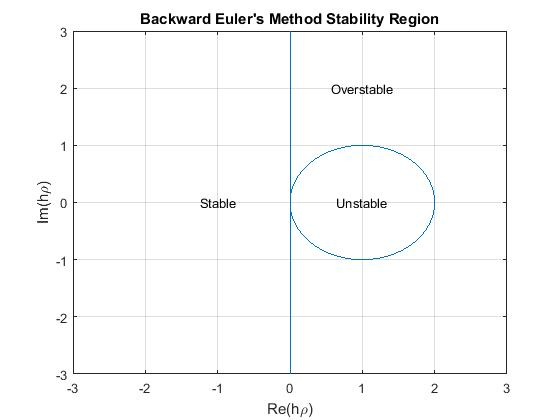
\includegraphics[width=100mm]{GraphEulerB.jpg}
					\centering
   					\caption{BE stability region}
				           \label{fig4}
  				\end{figure}

Now we will proceed to determine if the forward and backward Euler's methods applied to the equation of motion lie within their respective stability regions or not. By uncoupling the equation of motion, we can analyze the individual modes of the system by just considering the mode that produces maximum amplifiaction; that is we consider the spectral radius $\rho$. The equation of motion system can be uncoupled into 
				\begin{figure}[h!]
   					\centering
   					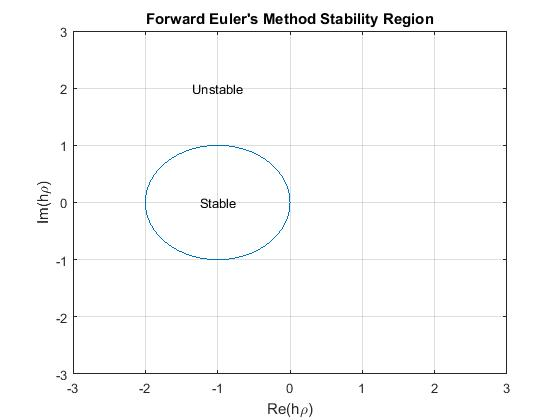
\includegraphics[width=100mm]{GraphEulerF.jpg}
					\centering
   					\caption{FE stability region}
				           \label{fig5}
  				\end{figure}

				\begin{equation}
					a_n + \xi\omega v_n + \omega^2 d_n = \phi_n
				\end{equation}
by looking at each different mode of the motion. Here $\omega^2$ is the stiffness coefficient and $\xi \omega$ is the dampnesss coefficient.
Thereby the amplification matrix is $\textbf{A} = \begin{bmatrix}0 & 1 \\ -\omega^2 & -\xi\omega \end{bmatrix}$ and $\L_n = \begin{bmatrix}\phi_n \\ 0 \end{bmatrix}$. Finding the characteristic equation of the amplification matrix $\textbf{A}$ will result in the eigenvalues that we are looking for:

				\begin{equation}
					\lambda^2 -\xi\omega\lambda + \omega^2 = 0
				\end{equation}
Hence 

				\begin{equation}
					\lambda_{1,2} = \frac{\xi\omega \pm \sqrt{\xi^2\omega^2 - 4\omega^2}}{2}
				\end{equation}
which has to satisfy the condition $\xi^2\omega^2-4\omega^2 < 0$ in order to have a complex solution which we are looking for. This condition reduces to $\xi < 2$ for

				\begin{equation}
					\lambda_{1,2} = \omega\left(\frac{\xi \pm i\sqrt{4 - \xi^2}}{2}\right)
				\end{equation}
Comparing (54) with figures (4) and (5) we see that the values of $h\lambda$ are in the unstable region for the Forward Euler method and generally in the overstable region for the Backward Euler method. In regards to accuracy Euler's method can be viewed as a special case of the Taylor series

				\begin{equation}
					y(x_{n+1}) = y(x_{n}) + h\dot{y}(x_{n}) + \frac{h^2}{2}\ddot{y}(c)
				\end{equation}
where $x_{n} < c < x_{n+1}$. The value of $c$ exits theoretically but in practice is unknown, but a bound on the error can be expressed as $\frac{Mh^2}{2}$, where $M = \text{max}_{x_{n} < x < x_{n+1}} |\ddot{y}|$. The truncation error is of order 2 denoted $O(h^2)$. In addition to truncation error (an error due to the method itself), there also exists round-off error which is due to the computation and the limited computer capacity to store decimal places. 

%%%%%%%%%%%%%%%%%%%%%%%%%%%%%%%%%%%%%%%%%%%%%%%%%%% NEWMARK DERIV

	\subsection{Newmark  Method}

		\subsubsection{Derivation}

			\paragraph{}A method for numerical integration that is widely used in structural dynamics applications is the Newmark method. It is a general method that can be used to solve any system of differential equations of the form:

				\begin{equation}
					\\
					\textbf{M}\ddot{X}+\textbf{C}\dot{X}+\textbf{K}X =F
					\\
				\end{equation}
subject to 

				\begin{align*}
					X(0)&=D_0\\
					\dot{X}(0)&=V_0
				\end{align*}
where $X$ and its derivatives are vector functions of time $t$. The Newmark method can be derived from the Taylor series expansion:

				\begin{equation}
					f(x) = f(a) + f'(a) \left( x-a \right)+{\frac { f''(a) \left( x-a \right) ^{2}}{2!}}+{\frac { f'''(a) \left( x-a \right) ^{3}}{3!}}+...+{\frac { f^{(n)}(a) \left( x-a \right) ^{n}}{n!}}
				\end{equation}
setting $h = x-a$ we get the more convenient form

				\begin{equation}
					f(x+h) = f(x) + f'(x)h +{\frac { f''(x) h ^{2}}{2}}+{\frac { f'''(x) h^{3}}{3!}}+...+{\frac { f^{(n)}(x)  h^{n}}{n!}}\\
				\end{equation}
and taking the derivative gives

				\begin{equation}
					f'(x+h) = f'(x) + f''(x)h +{\frac { f'''(x) h ^{2}}{2}}+{\frac { f^{(4)}(x) h^{3}}{3!}}+...+{\frac { f^{(n)}(x)  h^{n}}{n!}}\\
				\end{equation}
$h$ is used as the time step in discrete physical applications such as ours, so the following hold true:

				\begin{align*}
					&h=\Delta t\\
					&f \left( x \right) =d_{{n}}\\
					&f \left( x+h \right) =d_{{n+1}}\\
					&f'(x) =v_{{n}}\\
					&f'(x+h) =v_{{n+1}}\\
					&f''(x) =a_{{n}}\\
					&f''(x+h) =a_{{n+1}}\\
					&\dot{a_{{n}}}=\frac {a_{{n+1}}-a_{{n}}}{\Delta t}	
				\end{align*}
To obtain an algorithm for displacement and velocity we truncate the Taylor series for displacement at the 4th term and the Taylor series for velocity at the 3rd term. The constants $\beta$ and $\gamma$ determine the stability and accuracy of the algorithm.

				\begin{align*}
				&D_{n+1} = D_{n}+V_{n}\Delta t+\frac{A_{{n}}{\Delta t}^{2}}{2}+2\beta \dot{A}_{n}{\Delta t}^3\\
				&D_{n+1} = D_{n}+V_{n}\Delta t+\frac{A_{{n}}{\Delta t}^{2}}{2}+2\beta (\frac {A_{{n+1}}-A_{{n}}}{\Delta t}){\Delta t}^3\\
				&D_{n+1} = V_{n}+V_{n}\Delta t+\frac{{\Delta t}^{2}}{2}[(1-2\beta)A_n + 2\beta A_{n+1}]\\ \\
				&V_{n+1} = V_{n}+A_{n}\Delta t+\gamma \dot{A}_{n} \Delta t^2\\
				&V_{n+1} = V_{n}+A_{n}\Delta t+\gamma(\frac{A_{n+1} - A_n}{\Delta t}){\Delta t}^2\\
				&V_{n+1} = V_{n}+\Delta t[(1-\gamma)A_n + \gamma A_{n+1}]
				\end{align*}
To summarize, the equation of motion (1) has been discretized into:

				\begin{equation}
					\\
					\textbf{M}A_{n+1}+\textbf{C}V_{n+1}+\textbf{K}X_{n+1} =F_{n+1}
					\\
				\end{equation}

				\begin{equation}
					D_{n+1} = D_{n}+v_{n}\Delta t+\frac{{\Delta t}^{2}}{2}[(1-2\beta)A_n + 2\beta A_{n+1}]
				\end{equation}

				\begin{equation}
					V_{n+1} = A_{n}+\Delta t[(1-\gamma)A_n + \gamma A_{n+1}]
				\end{equation}

%%%%%%%%%%%%%%%%%%%%%%%%%%%%%%%%%%%%%%%%%%%%%%%%%%%% NEWMARK IMPL
	
	\subsubsection{Implementation}
To compute the solution using this algorithm it is useful to define

				\begin{equation}
					\widetilde{D}_{n+1} = D_n+V_{n}h+\frac{\,{\Delta t}^{2}}{2} \left( 1-2\,\beta \right) A_{{n}}
				\end{equation}

				\begin{equation}
					\widetilde{V}_{n+1} = V_n+V_{n}h+\Delta t\, \left( 1-\gamma \right) a_{{n}}	
				\end{equation}
combining (61), (62) with (63), (64), respectively

				\begin{equation}
					D_{n+1} = \widetilde{D}_{n+1}+{\Delta t}^{2}\beta\,a_{{n+1}}
				\end{equation}

				\begin{equation}
					V_{{n+1}}=\widetilde{V}_{{n+1}} + \Delta t\,\gamma a_{{n+1}}
				\end{equation}
Substituting (65) and (66) into (60) we get
	
				\begin{equation*}
					\textbf{M}A_{{n+1}}+\textbf{C} \left(\widetilde{V}_{{n+1}}+\Delta t\gamma A_{{n+1}} \right) +\textbf{K} \left( {\Delta t}^{2}\beta\,A_{{n+1}}+\textbf{D}_{{n+1}} \right) =F_{{n+1}}
				\end{equation*}
and after factoring, 

				\begin{equation}
					\left(\textbf{K}{\beta \Delta t}^{2}+\textbf{C}\Delta t\gamma +\textbf{M} \right) A_{{n+1}}=-\textbf{C}\widetilde{V}_{{n+1}}-\textbf{K}\widetilde{D}_{{n+1}}+F_{{n+1}}
				\end{equation}
Therefore, one possible implementation is to calculate (63) and (64), solve for $A_{n+1}$ in (67) and use (65) and (66) to determine the next $D$ and $V$.
\newline \newline
				\begin{center}
					\framebox{
					\parbox[t][7.5cm]{10cm}{
					\addvspace{0.2cm} \centering 
					\begin{center} Implementation 1\end{center}
					\begin{align*}
				&1. \ \text{Using initial conditions $d_0$ and $v_0$ calculate $a_0$}\\
				&\ A_{{0}}= \textbf{M}^{-1} (F_{{0}}-\textbf{C}V_{{0}}-\textbf{K}D_{{0}} )\\
			           &\text{For each $ith$ term in the $d$, $v$ and $a$ vectors do the following:}\\
				&2. \  \widetilde{D}_{n+1} = D_n + V_n\Delta t+\frac{\,{\Delta t}^{2}}{2} \left( 1-2\,\beta \right) A_{{n}}\\
				&3. \  \widetilde{V}_{{n+1}}=V_{{n}}+\Delta t\, \left( 1-\gamma \right) A_{{n}}\\
				&4. \  A_{{n+1}}= [ \textbf{M} +\textbf{C} \gamma \Delta t + \textbf{K} \beta {\Delta t}^2]^{-1}[F_{{n+1}} -\textbf{C} \widetilde{V}_{n+1} - \textbf{K}\widetilde{D}_{n+1}]\\
				&5. \  D_{n+1} = \widetilde{D}_{n+1} + {\Delta t}^{2}\beta\,A_{{n+1}}\\
				&6. \  V_{{n+1}}=\widetilde{V}_{{n+1}}+\Delta t\,\gamma A_{{n+1}}\\
				&\text{Repeat steps 2. through 6. for the entire vector length}
					\end{align*}
} 
}\newline 
				\end{center}
Here $\widetilde{D}_{{n+1}}$ and $\widetilde{V}_{{n+1}}$ are known as predictors and $D_{{n+1}}$ and $V_{{n+1}}$. By using (65) and (66) to eliminate $V_{n+1}$ and $A_{n+1}$ from (60) another possible implementation can be made. 

			\begin{align*}
				&A_{{n+1}}={\frac {D_{{n+1}}-\widetilde{D}_{{n+1}}}{{\Delta t}^{2}\beta}}\\
				&V_{{n+1}}=\widetilde{V}_{{n+1}}+\Delta t\,\gamma \left( {\frac {D_{{n+1}}-\widetilde{D}_{{n+1}
}}{{\Delta t}^{2}\beta}} \right) \\
				&\textbf{M} \left( {\frac {D_{{n+1}}-\widetilde{D}_{{n+1}}}{{\Delta t}^{2}\beta}} \right) +\textbf{C}\left[{{\widetilde{V}_{{n+1}}+\Delta t\,\gamma \left( {\frac {D_{{n+1}}-\widetilde{D}_{{n+1}}}{{\Delta t}^{2}\beta}} \right) }}\right]+\textbf{K}D_{{n+1}}=F_{{n+1}}\\
				&\left( {\frac {\textbf{M}}{{\Delta t}^{2}\beta}}+{\frac {\textbf{C}\gamma}{\Delta t\,\beta}}+\textbf{K} \right) D_{{n+1}}=F_{{n+1}}+\textbf{M} \left( {\frac {\widetilde{D}_{{n+1}}}{{\Delta t}^{2}\beta}} \right) -\textbf{C}\left({{\widetilde{V}_{{n+1}}-{\frac {\gamma \widetilde{D}_{{n+1}}}{\Delta t\,\beta}}}}\right)\\
				\\&\text{By using the expressions for $\widetilde{D}_{n+1}$ and $\widetilde{V}_{n+1} $}\\ \\
				&\widetilde{D}_{n+1} = D_{{n}} + V_n\Delta t+\frac{{\Delta t}^{2}}{2}\left( 1-2\,\beta \right) A_{{n}}\\
				&\widetilde{V}_{{n+1}}=A_{{n}}+\Delta t\, \left( 1-\gamma \right) A_{{n}}\\
				\\&D_{n+1} \ \text{can be isolated in terms of only the previous time step vectors}\\ \\
				&{\frac {\widetilde{D}_{{n+1}}}{{\Delta t}^{2}\beta}} = \frac{D_n}{\beta {\Delta t}^2} + \frac{V_n}{\beta \Delta t} + \left(\frac{1}{2\beta} - 1\right)A_n\\
				&\widetilde{V}_{{n+1}}-{\frac {\gamma \widetilde{D}_{{n+1}}}{\Delta t\,\beta}} = -{\frac {\gamma D_{{n}}}{\Delta t\beta }}+ \left( 1-{\frac {\gamma}{\beta}} \right) V_{{n}}+\Delta t \left( 1-{\frac {\gamma}{2\beta}}
 \right) A_{{n}}
			\end{align*}
\begin{center}
\framebox{
\parbox[t][15.5cm]{10cm}{
\addvspace{0.2cm} \centering 
			\begin{center} Implementation 2\end{center}
			\begin{align*}
				&1. \ \text{Using initial conditions $D_0$ and $V_0$ calculate $A_0$}\\
				&\ A_{{0}}= \textbf{M}^{-1} (F_{{0}} -\textbf{C}V_{{0}}-\textbf{K}D_{{0}})\\
				\\ &2. \ \text{Define constants}\\
				&\ \ \ \ \ c_1 = {\frac {1}{{\beta \Delta t}^{2}}}\\
				&\ \ \ \ \ c_2 =\frac{1}{\beta \Delta t }\\	
				&\ \ \ \ \ c_3 = \frac{1}{2\beta}-1\\	
				&\ \ \ \ \ c_4 = \frac {\gamma}{\beta \Delta t}\\	
				&\ \ \ \ \ c_5 = 1-{\frac {\gamma}{\beta}}\\	
				&\ \ \ \ \ c_6 = \Delta t \left( 1-{\frac {\gamma}{2\beta}} \right) \\	
				\\ &3. \ \text{Define inverted matrix allowing for explicit calculation of $d_{n+1}$}\\
				&\textbf{W}=\left[{\frac {\textbf{M}}{{\Delta t}^{2}\beta}}+{\frac {\textbf{C}\gamma}{\Delta t\,\beta}}+\textbf{K}\right]^{-1}\\
				\\ &4. \ \text{For each time step calculate $D_{n+1}$, $V_{n+1}$ and $A_{n+1}$}\\
				&\widetilde{A}_{{n+1}}=-c_1D_n+c_2V_n+c_3A_n\\
				&\widetilde{V}_{{n+1}}=c_4D_n+c_5V_n+c_6A_n\\
				&D_{{n+1}}=\textbf{W}[F_{{n+1}}+\textbf{M}\widetilde{A}_{{n+1}}-\textbf{C}\widetilde{V}_{{n+1}}]\\
				&V_{n+1} = c_4D_{n+1}+\widetilde{V}_{{n+1}}\\
				&A_{n+1}= c_1D_{n+1}-\widetilde{A}_{{n+1}}
			\end{align*}
} 
} \newline \newline \newline
\end{center}
This latter implementation is more used in practice as it entails one less stiffness calculation than Implementation 1.

%%%%%%%%%%%%%%%%%%%%%%%%%%%%%%%%%%%%%%%%%%%%%%%%%%%% STAB ANALYSIS

	\subsubsection{Stability Analysis}

				\paragraph{Amplification matrix} To analyze the stability of the Newmark method we write down the discrete equation of motion for $t_n$ and $t_{n+1}$, 

				\begin{equation}
					\textbf{M}A_{n}+\textbf{C}V_{n}+\textbf{K}X_{n} =F_{n}\\
				\end{equation}

				\begin{equation}
					\textbf{M}A_{n+1}+\textbf{C}V_{n+1}+\textbf{K}X_{n+1} =F_{n+1}
				\end{equation}
 After multiplying (63) and (64) by $\textbf{M}$ and substituting the above two equations we get the relations

				\begin{equation*}
					\textbf{M}D_{n+1} = \textbf{M}D_{n} + \textbf{M}V_{n}\Delta t + \newline \frac{\Delta t^2}{2}\left[(1 - 2\beta)(-\textbf{C}V_n - \textbf{K}D_n + F_n) + 2\beta(-\textbf{C}V_{n+1}- \textbf{K}D_{n+1} + F_{n+1})\right]
				\end{equation*}

				\begin{equation*}
					\textbf{M}V_{n+1} = \textbf{M}V_{n} + \newline \Delta t\left[(1 - \gamma)(-\textbf{C}V_n - \textbf{K}V_n + F_n) + \gamma(-\textbf{C}V_{n+1}- \textbf{K}D_{n+1} + F_{n+1})\right]
				\end{equation*}
Written in matrix form we have the amplification matrix $\textbf{A}$
	
				\begin{equation}
					U_{n+1} = \textbf{A}U_n
				\end{equation}
where 

				\begin{equation}
					\textbf{A} = \textbf{A}_1^{-1}\textbf{A}_2
				\end{equation} \newline

				\begin{equation}
					\textbf{A}_1 = \begin{bmatrix} \textbf{M}+ \textbf{K} \beta \Delta t^2 & \textbf{C} \beta \Delta t^2 \\
\textbf{K} \gamma \Delta t & \textbf{M} + \textbf{C}\gamma \Delta t\end{bmatrix} 
				\end{equation} \newline

				\begin{equation}
					\textbf{A}_2 = 
						\begin{bmatrix} 
						\textbf{M}- \textbf{K}(1 - 2\beta)\frac{\Delta t^2}{2} & \textbf{M} \Delta t -  \textbf{C}(1 - 2\beta)\frac{\Delta t^2}{2} \\
						\textbf{K}(\gamma - 1)\Delta t & \textbf{M} - \textbf{C}(1 - \gamma)\Delta t
						\end{bmatrix}
				\end{equation} \newline



%%%%%%%%%%%%%%%%%%%%%%%%%%%%%%%%%%%%%%%%%%%%%%%% NEWMARK UNDAMP STAB
				\paragraph{Undamped motion} Consider the undamped equation of motion

				\begin{equation}
					\textbf{M}\ddot{X}+\textbf{K}X =F
				\end{equation}
				The system is composed of the uncoupled equations of the form

				\begin{align}
				&a_n + \omega^2 d_n = \phi_n\\
				&a_{n+1} + \omega^2 d_{n+1} = \phi_{n+1}
				\end{align}
where $\omega^2$ is the square of the natural frequency of a given floor and an eigenvalue of a stiffness matrix $\textbf{Q} = \textbf{M}^{-1}\textbf{K}$, and $\phi_n$ is a factor depending on the force of the earthquake and its effect on a particular floor. Applying (77) and (78) to (70) we get

				\begin{equation}
					\textbf{A} = 
						\begin{bmatrix} 
						1+ \beta \Delta t^2 \omega^2 & 0 \\
						\gamma \Delta t \omega^2& 1\end{bmatrix}^{-1}\begin{bmatrix} 1 - (1 - 2\beta)\frac{\Delta t^2}{2}\omega^2 & \Delta t \\
					(\gamma - 1)\Delta t \omega^2 & 1
					\end{bmatrix}
				\end{equation}

				\begin{equation}
					\textbf{A} = \begin{bmatrix} 1 - \frac{1}{2} \frac{\Omega^2}{T} & \frac{\Delta t}{T}  \\
-\Omega \omega \left( 1 - \frac{\gamma}{2} \frac{\Omega^2}{T}\right)& 1 - \gamma \frac{\Omega^2}{T} \end{bmatrix}
				\end{equation}
where $\Omega = \Delta t \omega$ and $T = 1+\beta \Omega^2$. Let $\epsilon^2 = \frac{\Omega^2}{T}$, so that the characteristic equation to find the eigenvalues of $\textbf{A}$ is

				\begin{equation}
					\lambda^2 - \lambda \left[2 - (\gamma + \frac{1}{2})\epsilon^2\right] + 1 - (\gamma - \frac{1}{2})\epsilon^2 =0
				\end{equation}
We consider only complex-conjugate eigenvalues, since we are interested in the physical reality - the equation of motion will be a vibration, and not a exponential increase. The condition for complex eigenvalues of (70) is

				\begin{equation}
					(\gamma + \frac{1}{2})^2 - 4\beta \leq \frac{4}{\Omega^2}
				\end{equation}
and the eigenvalues are

				\begin{equation}
					\lambda_{1,2} = \rho e^{\pm i\phi}
				\end{equation}
where 

				\begin{equation*}
					\rho = \sqrt{1- (\gamma - \frac{1}{2})\epsilon^2}
				\end{equation*}
				
				\begin{equation*}
					\phi = \tan^{-1}\left( \frac{\epsilon \sqrt{1- \frac{1}{4}(\gamma + \frac{1}{2})^2\epsilon^2}}{1-\frac{1}{2}(\gamma +\frac{1}{2})\epsilon^2}\right)
				\end{equation*}
Therefore, to ensure that the method is stable ($\rho \leq 1$) the following condition must be ensured

				\begin{equation}
					\gamma \geq \frac{1}{2}
				\end{equation}
and that 

				\begin{equation}
					(\gamma + \frac{1}{2})^2 - 4\beta \leq \frac{4}{\Omega_i^2}
				\end{equation}
for each $i = 1 \dots N$. Furthermore the method become unconditionally stable if in addtion to (82) of the following condition is met

				\begin{equation}
					\beta \geq \frac{1}{4}\left(\gamma + \frac{1}{2}\right)^2
				\end{equation}
For $\gamma = \frac{1}{2}$ and $\beta = \frac{1}{4}$ the method becomes unconditionally stable and has the highest degree of accuracy. This is known as the average constant acceleration method or the trapezoidal rule.

				\begin{figure}[h!]
   					 \centering
   					 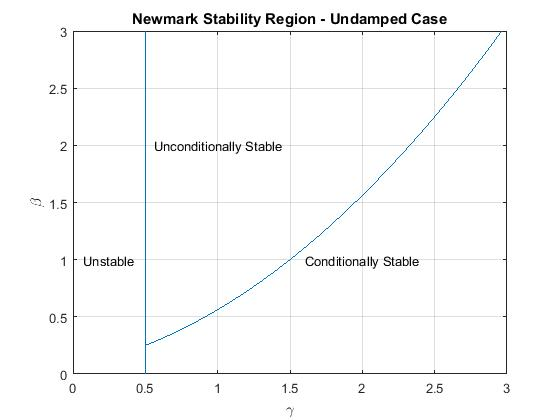
\includegraphics[width=90mm]{GraphNM.jpg}
   					 \caption{Newmark Method Stability Regions}
				            \label{fig6}
  				\end{figure}

%%%%%%%%%%%%%%%%%%%%%%%%%%%%%%%%%%%%%%%%%%%%%%%%% NEWMARK DAMP STAB
			\paragraph{Damped motion} Consider the modal decomposition of the damped equation of motion

				\begin{equation*}
					a_n + 2\xi\omega v_n + \omega^2 d_n = \phi_n
				\end{equation*}
In order to simplify matters, let's choose $\gamma = \frac{1}{2}$ and $\beta = \frac{1}{4}$ thereby the amplification matrix becomes

				\begin{equation*}
					\textbf{A} = \begin{bmatrix} 1+ \frac{\Delta t^2 \omega^2}{4} & \frac{\Delta t^2 \xi \omega}{2} \\
\frac{\Delta t \omega^2}{2}& 1 + \Delta t \xi \omega\end{bmatrix}^{-1}\begin{bmatrix} 1 -\frac{\Delta t^2 \omega^2}{4} & \Delta t -  \frac{\Delta t^2 \xi \omega}{2} \\ -\frac{\Delta t \omega^2}{2} & 1 - \Delta t \xi \omega \end{bmatrix}
				\end{equation*}

Setting the det($\textbf{A}-\lambda \textbf{I}$) = 0 the characteristic equation becomes

				\begin{equation*}
					\lambda^2\left( 1 + \Delta t \xi \omega + \frac{\Delta t^2 \omega^2}{4}\right) - 2\lambda\left( 1 - \frac{\Delta t^2 \omega^2}{4} \right) + \left(1 - \Delta t \xi \omega + \frac{\Delta t^2 \omega^2}{4}\right)  = 0
				\end{equation*}
If $\xi<1$, then the roots remain complex and the spectral radius remains below 1. In general damping has a beneficial effect by increasing the stability.



%%%%%%%%%%%%%%%%%%%%%%%%%%%%%%%%%%%%%%%%%%%%%%%%%%%%%% EXAMPLES
%%%%%%%%%%%%%%%%%%%%%%%%%%%%%%%%%%%%%%%%%%%%%%%%%%%%%%%%%%%
	
\section{Examples}

	\subsection{Simple cases}

				\paragraph{2-Floor case} A very simple example will allow for an overview of all the methods of solution that were discussed previously. Let there be a 2-story building with each floor having a mass of 10,000 kg and a spring constant 20,000 $\frac{\text{kg}}{\text{s}^2}$. To simulate an earthquake we will make the first floor move with 0.2 $\frac{\text{m}}{\text{s}}$ at the beginning. We will proceed to solve this analytically and afterwards compare the solution to the numerical methods. 
\newline
\newline
The matrix $\textbf{H}$ which turns the second-order problem into a first order problem is 

				\begin{equation*}
					\textbf{H} = \begin{bmatrix}0&0&1&0\\0&0&0&1\\-4&2&0&0\\2&-2&0&0\end{bmatrix}
				\end{equation*}
The eigenvalues of $\textbf{H}$  are 2.2882i, -2.2882i, 0.8740i and -0.8740i. This illustrates that an even n-by-n matrix with 0 upper-left and identity upper-right submatrices will have eigenvalues that come in conjugate pairs. Physically we are just interested in the positive eigenvalue of the conjugate pair; the eigenvalues correspond to the natural frequencies of the building. The corresponding eigenvectors are the column vectors of matrix $\textbf{P}$

				\begin{equation*}
					\textbf{P} = \begin{bmatrix}-0.3406i&0.3406i&-0.3958&0.3958\\0.2105i&-0.2105i&-0.6405&-0.6405\\0.7795&0.7795&-0.3460i&0.3460i\\-0.4817&-0.4817&-0.5598i&0.5598i\end{bmatrix}
				\end{equation*}
The eigenvectors are complex conjugate pairs and we use the first and third eigenvalues and eigenvectors to form the solution. Using the initial condition and equations (8) and (9) the exact analytical solution is found

				\begin{align*}
					U = &c_1\left[\text{Re}(A)\cos{\alpha t} -\text{Im}(A)\sin{\alpha t}\right]+c_2\left[\text{Re}(A)\cos{\alpha t} -\text{Im}(A)\sin{\alpha t}\right] \\ + &c_3\left[\text{Re}(B)\cos{\beta t} -\text{Im}(B)\sin{\beta t}\right]+c_4\left[\text{Re}(B)\cos{\beta t} -\text{Im}(B)\sin{\beta t}\right]
				\end{align*}
where $U$ is the general solution, $A$ is the first column vector of $\textbf{P}$ and $B$ is the second column vector of $\textbf{P}$. When solving for the initial condition $U(0) = \begin{bmatrix}0\\0\\0.2\\0\end{bmatrix}$ the constants $c_1$ and $c_2$ become 0 and the solution becomes

				\begin{equation*}
					U = c_1\left[\text{Re}(A)\cos{\alpha t} -\text{Im}(A)\sin{\alpha t}\right]+c_4\left[\text{Re}(B)\cos{\beta t} -\text{Im}(B)\sin{\beta t}\right]
				\end{equation*}
where $\alpha = 2.2882$, $\beta = 0.8740$, $c_1 = 0.1857$, $c_2 = -0.1598$. Figures \ref{fig7} and \ref{fig8} compare the Analytical solution with the Newmark method and the Backward Euler method. As we can see the Backward Euler method starts very close to the actual solution but diverges from it farther and farther with increasing time.

				\begin{figure}[h!]
  					\centering
 				 	\begin{minipage}[b]{0.4\textwidth}
    						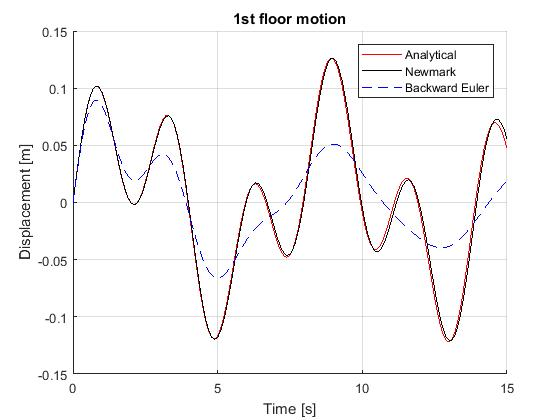
\includegraphics[width=90mm]{1floor.jpg}
						\caption{1st floor motion}
						\label{fig7}
  					\end{minipage}
 					 \hfill
					\begin{minipage}[b]{0.4\textwidth}
 				  	 	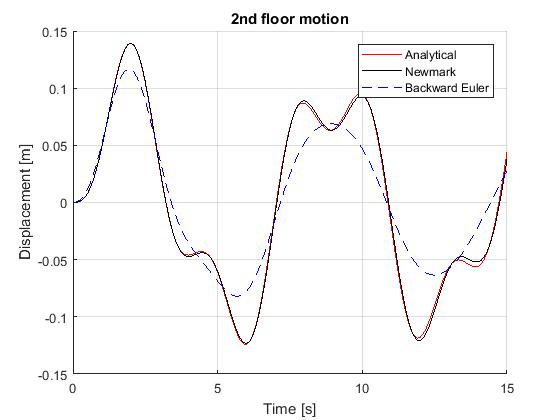
\includegraphics[width=90mm]{2floor.jpg}
						\caption{2nd floor motion}
						\label{fig8}
 					 \end{minipage}
				\end{figure}
In the example we used the same time step for the Euler method as for the Newmark method (specifically we used $\Delta t = 0.1$). If we decrease the time step for the Euler method we will approach the true solution to farther into time. This shows another benefit of the Newmark method - relatively high accuracy for large time steps. In this particular example an Euler method with $\Delta t = 0.001$ was about as accurate as the Newmark method with time step $\Delta t = 0.1$ (see Figure \ref{fig9}). 
				\begin{figure}[h!]
   					 \centering
   					 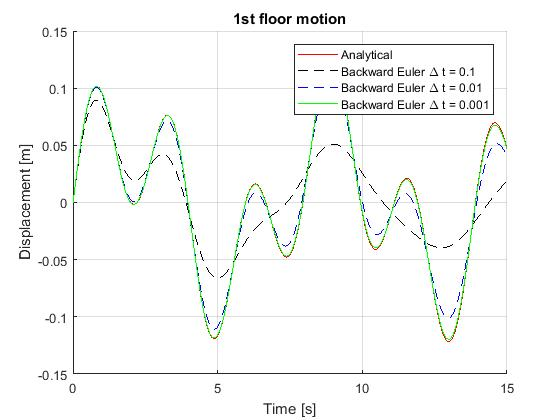
\includegraphics[width=90mm]{Eulerdiff.jpg}
   					 \caption{Euler method approaching solution at different time steps}
				            \label{fig9}
  				\end{figure}

				\paragraph{10-Floor case} Let's look at the same building parameters as in the first case (10000 kg floors and 20000 $\frac{\text{kg}}{\text{s}^2}$). In this case we will just find the eigenvalues of the stiffness matrix and make a conclusion about the stability of the building. The stiffness matrix $\textbf{G} = \textbf{M}^{-1}\textbf{K}$ is 

				\begin{equation*}
					\textbf{Q}=  \begin{bmatrix}-4&2&0&0&0&0&0&0&0&0\\2&-4&2&0&0&0&0&0&0&0\\0&2&-4&2&0&0&0&0&0&0\\0&0&2&-4&2&0&0&0&0&0\\0&0&0&2&-4&2&0&0&0&0\\
				  0&0&0&0&2&-4&2&0&0&0\\0&0&0&0&0&2&-4&2&0&0\\0&0&0&0&0&0&2&-4&2&0\\0&0&0&0&0&0&0&2&-4&2\\0&0&0&0&0&0&0&0&2&-2\end{bmatrix}
				\end{equation*}
The eigenvalues of the 20-by-20 compound matrix of the form $\textbf{H} = \begin{bmatrix} \textbf{0} & \textbf{I} \\ -\textbf{G} &-\textbf{Q}\end{bmatrix}$, with $\textbf{Q}=\textbf{0}$ (since there is no damping) are the frequencies of each floor starting from the bottom to the top. To find the resonating period of each floor we use the relationship $T=\frac{2\pi}{\lambda}$. This yields the following values

				\begin{center}
    					\begin{tabular}{| l | l | l | l |}
    \hline
    Floor & Eigenvalue, $\lambda$ [$s^{-1}$] & Period, $T$ [s] \\ \hline
    1 & 2.7968 & 2.2465 \\ \hline
    2 & 2.7028 & 2.3247 \\ \hline
    3 & 2.5483 & 2.4656 \\ \hline
    4 & 2.3370 & 2.6886 \\ \hline
    5 & 2.0734 & 3.0304 \\ \hline
    6 & 1.7635 & 3.5629 \\ \hline
    7 & 1.4142 & 4.4429 \\ \hline
    8 & 1.0333 & 6.0805 \\ \hline
    9 & 0.6294 & 9.9831 \\ \hline
   10 & 0.2114 & 29.7262 \\ \hline
   					 \end{tabular}
				\end{center}
Typical earthquakes have periods of 2-3 seconds which means that the lower floors of the builidng in the example are in danger of developing resonance with the earthquakes frequency. 

%%%%%%%%%%%%%%%%%%%%%%%%%%%%%%%%%%%%%%%%%%%%%%%%%%%%%% EL CENTRO
	\subsection{El Centro Earthquake}
In 1940 an earthquake occurred in the Imperial Valley in California. It became known as the El Centro Earthquake and was the first major earthquake to be recorded by a strong-motion seismograph located next to a fault line. The earthquake was characterized as a typical moderate-sized destructive event (maximum magnitude: 6.9 on the Richter Scale). It was the strongest recorded earthquake to hit the Imperial Valley, caused widespread damage to irrigation systems and led to the deaths of 9 people. The data from this earthquake will be used in the following examples to compare some the responses of different kinds of structures to earthquakes. Figure \ref{fig9} shows the acceleration of the ground as measured in 1940 in El Centro. 

				\begin{figure}[h!]
   					 \centering
   					 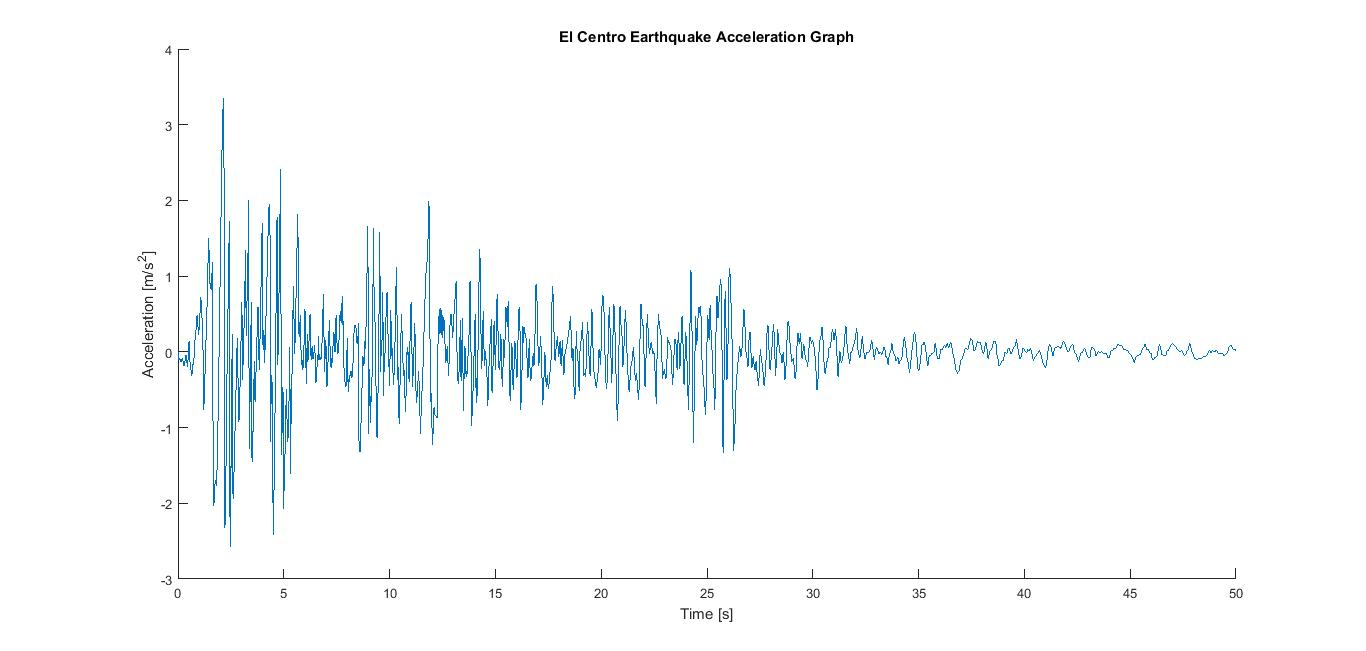
\includegraphics[width=180mm]{ElCentro.jpg}
   					 \caption{El Centro Acceleration Data}
				            \label{fig10}
  				\end{figure}

	\paragraph{2-Story Family House} Looking at the results from the simple cases and comparison of methods leads us to choose the Newmark method for the analysis of these real-world problems. First let's consider average 2-story houses made from wood as supporting material, typical for the region at this time. The mass of each floor will be assumed at 100,000 $kg$. This is based on the estimation of the weight of the concrete slab foundation and wooden material used for walls and ceilings. The stiffness constant can again be estimated using the relationship $k = \frac{AE}{L}$, where $A$ is cross-sectional area, $E$ is the elastic modulus, $L$ the length of the material. Again using estimation and wood as a material the stiffness constant is $12\text{x}10^5$ $\frac{kg}{s^2}$. The effect of the damping coefficient also estimated at $10^5$ $\frac{kg}{s}$ will be examined as compared to the motion of the building without a damping term. 

				\begin{figure}[h!]
   					\centering
   					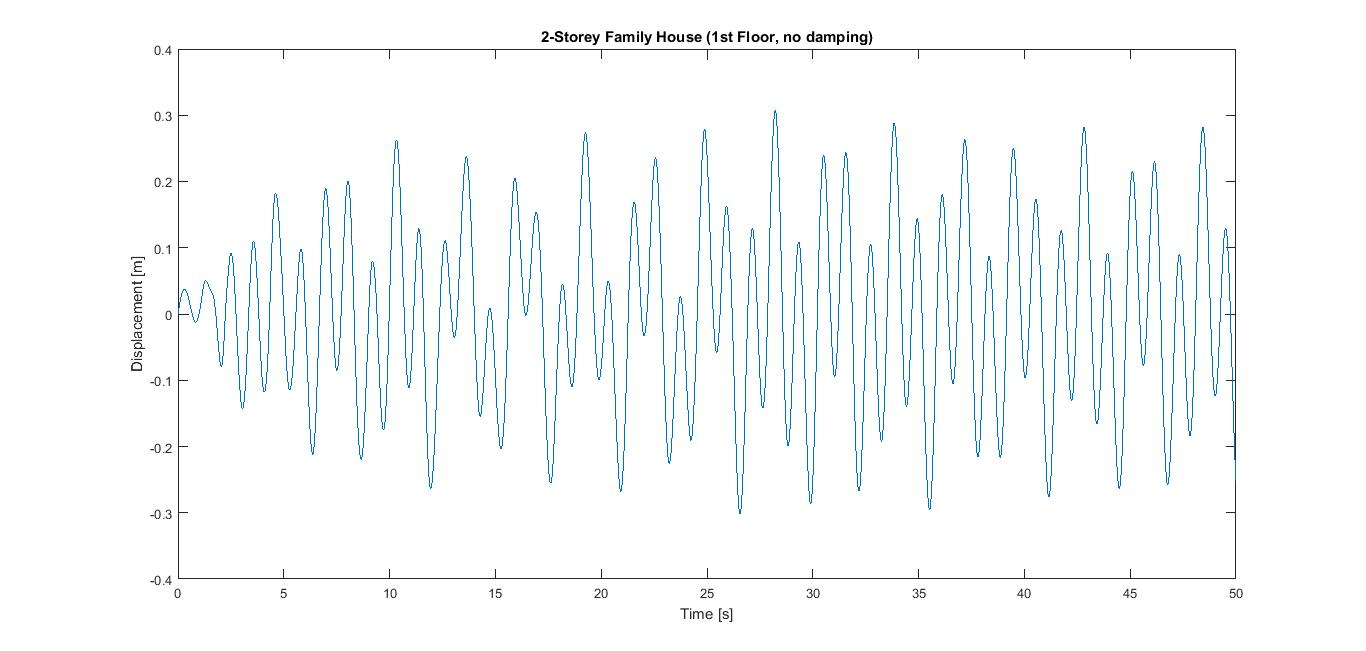
\includegraphics[width=142mm]{FM1.jpg}
					\caption{1st floor No Damping}
					\label{FM1}
  				\end{figure}

				\begin{figure}[h!]
   					\centering
					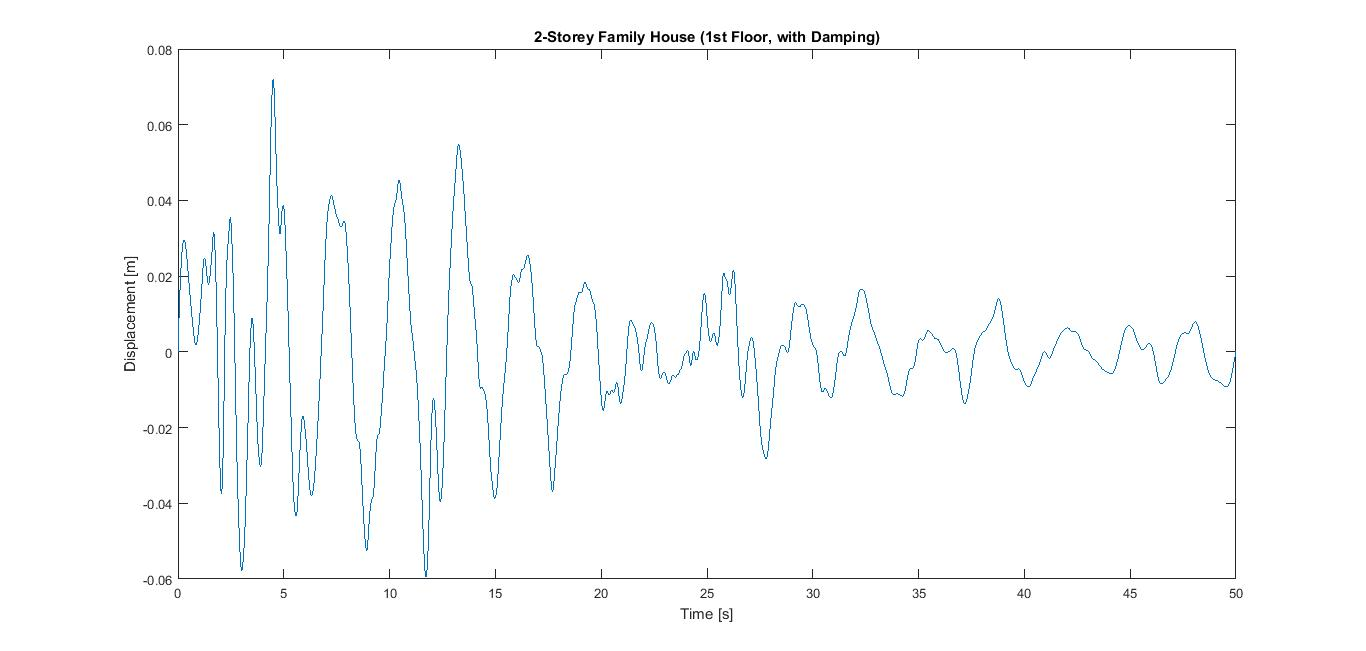
\includegraphics[width=142mm]{FMD1.jpg}
					\caption{1st floor Damping}
					\label{FMD1}
  				\end{figure}

	\paragraph{Skyscraper}As expected the damping term plays a very important role in the dynamics of the building, in fact lowering the maximal displacements 10-fold. Now we will look at the effects of the same earthquake on a skyscraper which will have a load-bearing structure out of steel. In this case using similar estimation techniques as for the 2-story case a 102 story building (height of the Empire State Building) will be tested for a response against the same earthquake data as before. Now a much higher mass - 3,600,000 $kg$ per floor is used and a much higher stiffness coefficient - 200x$10^6$ $\frac{kg}{s}$.
				

				\begin{figure}[h!]
   					\centering
   					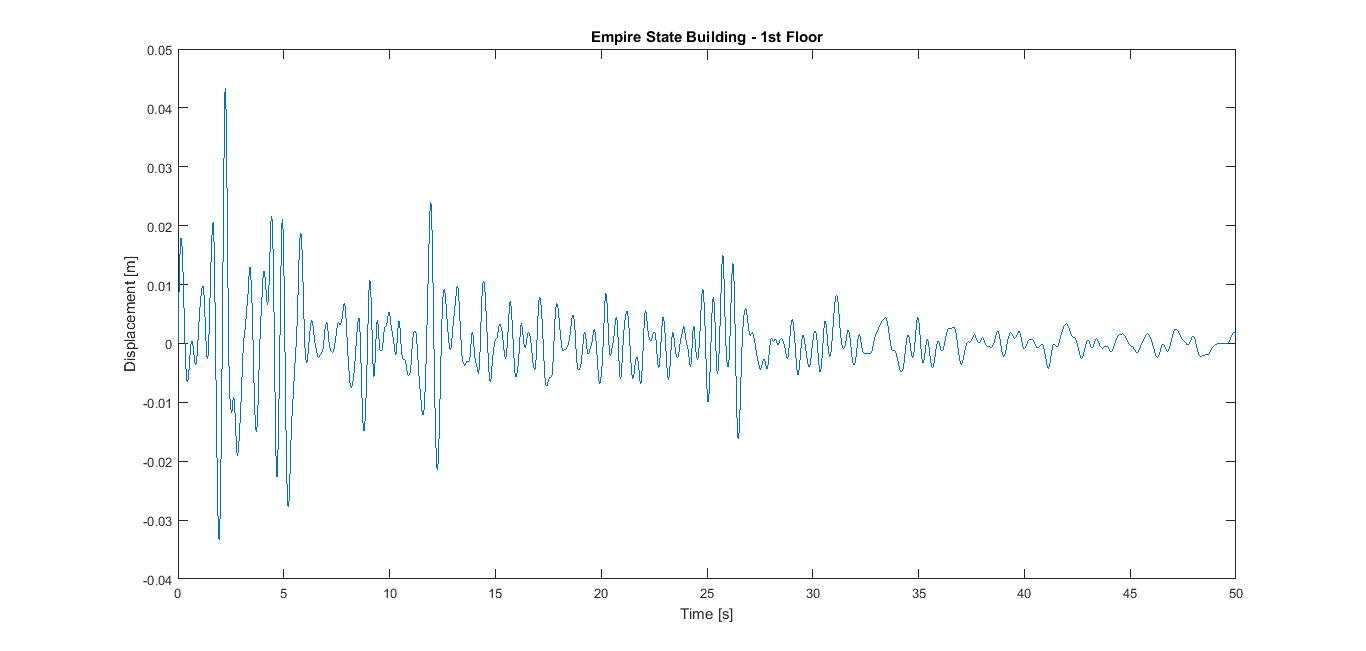
\includegraphics[width=142mm]{EmpireState.jpg}
					\caption{1st floor}
					\label{EmpireState}
  				\end{figure}

				\begin{figure}[h!]
   					\centering
					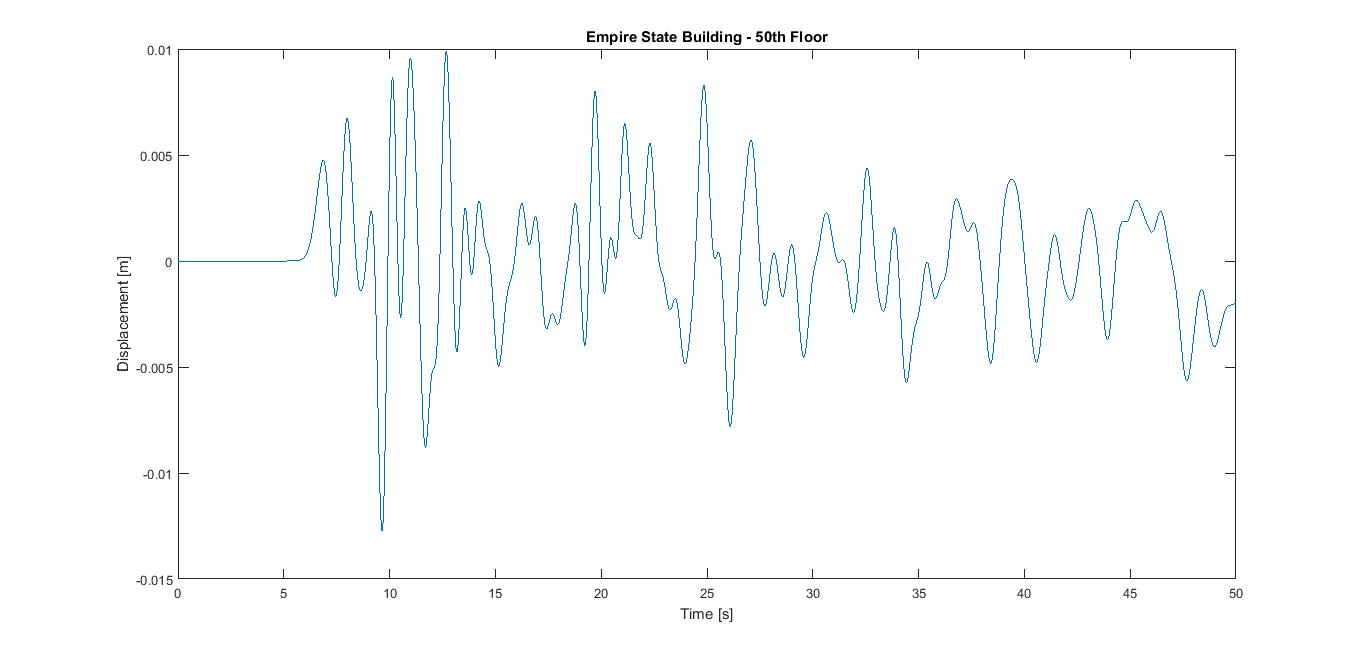
\includegraphics[width=142mm]{EmpireState50.jpg}
					\caption{50th floor}
					\label{EmpireState50}
  				\end{figure}

The maximum displacements of the tall structure are surprisingly a lot less than the displacements of the small 2-story house. The reason for this is the ratio of mass to stiffness coefficient which is 0.018 in the case of the skyscraper and 0.0833 in the case of the house. This is logical as we expect more massive and less elastic objects to have smaller displacements as compared to light and elastic objects. Another major reason is the range of the eigenvalues (natural frequencies) - the house had natural periods at 1.090 $s$ and 2.923 $s$ while the building had periods ranging from 0.5 to 6 but since there was no evident resonance it can be assumed that natural frequencies where very different from the periods of the earthquake.

%%%%%%%%%%%%%%%%%%%%%%%%%%%%%%%%%%%%%%%%%%%%%%%%%%%% STAB EXAMPLE

	\subsection{Stability example}
To see how the different parameters of the Newmark method influence the behavior of the solution we will consider two simple cases. We will examine the accuracy in a simple manner by comparing the analytical solution values with the numerical solution values. First consider the single second order differential equation

				\begin{equation*}
					\ddot{x} + x = 0
				\end{equation*}
with initial conditions $x(0) = 1$, $\dot{x}(0) = 0$. The exact solution is $x = \cos(t)$. 4 sets of parameters of the Newmark method will be checked: Unconditionally stable ($\gamma = 1$, $\beta = 1.5$), Conditionally stable ($\gamma = 2$, $\beta = 0.5$), Unstable($\gamma = 1$, $\gamma = 0.25$), Constant Acceleration ($\gamma = 0.5$, $\beta = 0.25$). The result is seen in the following graph

				\begin{figure}[h!]
   					 \centering
   					 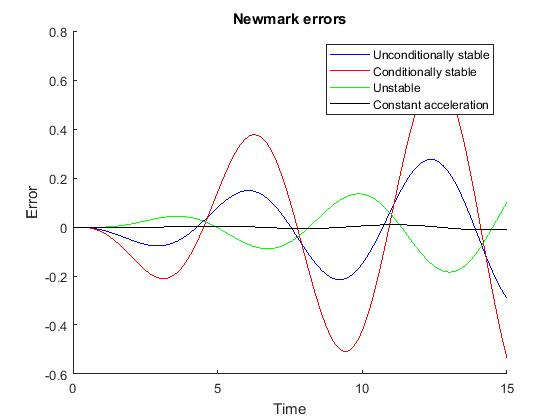
\includegraphics[width=90mm]{untitled.jpg}
   					 \caption{Errors in the Newmark method with different parameters}
				            \label{fig17}
  				\end{figure}
It can be seen from the graph that the Newmark method has the least amount of errors for Constant Acceleration method and the greatest errors for the conditionally stable method as opposed to the unstable method. This is a slightly surprising effect. However, if we look at the error as a combination of amplitude and period errors we will see that this occurrence is not by chance. We will refer to \cite{Gerardin} for the equations of the two types of errors.
\newline
\textbf{Amplitude error}
				
				\begin{equation*}
					\rho - 1 = -\frac{1}{2}\left( \gamma - \frac{1}{2} \right)\omega^2\Delta t^2 + O(\Delta t^4)
				\end{equation*}

\textbf{Periodicity errror}

				\begin{equation*}
					\frac{\Delta T}{T} =\frac{\omega \Delta t}{\phi} - 1 = \frac{1}{2}\left( \beta - \frac{1}{12} \right)\omega^2\Delta t^2 + O(\Delta t^3)
				\end{equation*}
Using equation (83) for the conditionally stable case we make a chart of the cases looked at

				\begin{center}
   					 \begin{tabular}{| l | l | l | l | l | l |}
						\hline & & & & &\\
	Algorithm & $\gamma$ & $\beta$ & Stability limit $\Omega$ & Amplitude error $\rho -1$ & Periodicity error $\frac{\Delta T}{T}$
						\\ & & & & &
						\\ \hline & & & & &\\
	Unconditionally stable & $1$ & $\frac{3}{2}$ & $\infty$ & $-\frac{\Omega^2}{4}$ & $\frac{17\Omega^2}{24}$
						\\ & & & & &\\
	Conditionally stable & 2 & $\frac{1}{2}$ & 0.97 &$-\frac{3 \Omega^2}{4}$ &  $\frac{5 \Omega^2}{24}$ 
						\\ & & & & &\\
	Unstable & 1 & $\frac{1}{4}$ & 0 & $-\frac{\Omega^2}{4}$ & $\frac{\Omega^2}{12}$ 
						\\ & & & & &\\
	Constant Acceleration & $\frac{1}{2}$ & $\frac{1}{4}$ & $\infty$ & $O(\Delta t^4)$ & $\frac{\Omega^2}{12}$ 
						\\ & & & & &\\
	Purely Explicit & 0 & 0 & 0 & $\frac{\Omega^2}{4}$ & $-\frac{\Omega^2}{24}$
						\\ & & & & &\\
	Linear Acceleration & $\frac{1}{2}$ & $\frac{1}{6}$ & 3.46 & $O(\Delta t^4)$ & $\frac{\Omega^2}{24}$
						\\ & & & & &\\ \hline
    					\end{tabular}
				\end{center}
From these results we can make the conclusion that the amplitude and periodicity errors are of order 2 (since $\Omega = \omega \Delta t$). We also see that the conditionally stable method with $\gamma = 2$ and $\beta = 0.5$ has the largest amplitude error which shows why this method was least accurate. 

%%%%%%%%%%%%%%%%%%%%%%%%%%%%%%%%%%%%%%%%%%%%%%%% CONVERGENCE EXAMPLE

	\subsection{Convergence Example}
The previous example leads us to conclude that the optimal parameters of the Newmark method are 

				\begin{equation*}
					\gamma = \frac{1}{2}
				\end{equation*}
to minimize the amplification error and

				\begin{equation*}
					 \frac{1}{12} \leq \beta \leq  \frac{1}{4}
				\end{equation*}
The beta value is in a range because for $\frac{1}{4}$ the method is conditionally stable, but for $\frac{1}{12}$ the periodicity error is minimized. Now we will use these parameters to examine the convergence behavior for the cases of conditional convergence ($ \frac{1}{12} \leq \beta <  \frac{1}{4}$). Using equation (83)

				\begin{equation*}
					\beta \geq \frac{1}{4}\left(\gamma + \frac{1}{2}\right)^2
				\end{equation*}
We plot the conditional stability limits and the errors, both of which are dependent on a choice for $\beta$. 

				\begin{figure}[h!]
   					 \centering
   					 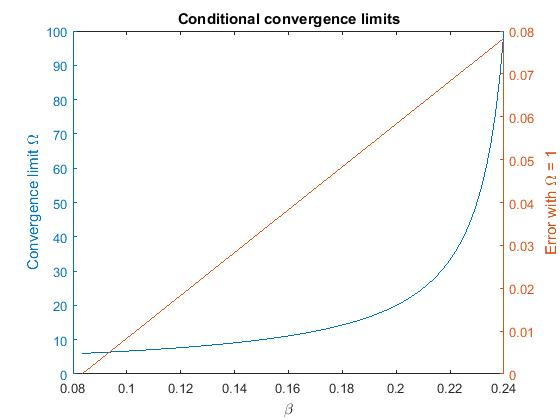
\includegraphics[width=90mm]{ccl3.jpg}
   					 \caption{Conditional stability limits and associated errors}
				            \label{fig17}
  				\end{figure}
The true periodicity error can be found by multiplying the points of the graph with the maximum $\Omega_1 = \omega_i\Delta t_i$ of the system.

%%%%%%%%%%%%%%%%%%%%%%%%%%%%%%%%%%%%%%%%%%%%%%%%%%%%% CONCLUSION

	\subsection{Conclusion}
By using numerical techniques and computational approaches to solving the dynamics problems associated with the motion of buildings during earthquakes it is possible to make estimates of the displacements of the building and design accordingly.


\section{Appendix}

				\paragraph{MATLAB Code} the following functions and scripts were used to implement the Euler, Runge-Kutta and Newmark methods as well as compute the examples and draw the graphs. 

\lstset{language=Matlab,%
    %basicstyle=\color{red},
    breaklines=true,%
    morekeywords={matlab2tikz},
    keywordstyle=\color{blue},%
    morekeywords=[2]{1}, keywordstyle=[2]{\color{black}},
    identifierstyle=\color{black},%
    stringstyle=\color{mylilas},
    commentstyle=\color{mygreen},%
    showstringspaces=false,%without this there will be a symbol in the places where there is a space
    numbers=left,%
    numberstyle={\tiny \color{black}},% size of the numbers
    numbersep=9pt, % this defines how far the numbers are from the text
    emph=[1]{for,end,break},emphstyle=[1]\color{red}, %some words to emphasise
    %emph=[2]{word1,word2}, emphstyle=[2]{style},    
}

	\subsection{Backward Euler Code}

		\lstinputlisting{Eulerb.m}

	\subsection{Runge-Kutta 4 Code}

		\lstinputlisting{RK4.m}

	\subsection{Newmark Code}

		\lstinputlisting{DynamicNewmark.m}


\begin{thebibliography}{9}

\bibitem{A first course in Differential Equations with Modeling Applications} 
Dennis G. Zill
\textit{Differential Equations and Their Applications}. 
Tenth Edition, Loyola Marymount University, Cengage Learning, 2012.

\bibitem{Hughes} 
Thomas J. R. Hughes.
\textit{The Finite Element Method: Linear Static and Dynamic Finite Element Analysis}. 
Chapter 9 Algorithms for Hyperbolic and Parabolic-Hyperbolic Problems, Dover Publications Inc., Mineola, New York, 2000.

\bibitem{Newmark} 
Nathan M. Newmark.
\textit{A Method of Computation for Structural Dynamics}. 
Journal of the Engineering Mechanics Divivsion, Proceedings of the American Society of Civil Engineers, 1959.

\bibitem{Gerardin} 
Michel G\'{e}rardin, Daniel Rixen
\textit{Mechanical Vibrations Theory and Application to Structural Dynamics}. 
Wiley, New York, 1994.

\bibitem{Faustett} 
Laurene V. Fausett
\textit{Applied Numerical Analysis Using MATLAB}. 
Second Edition, Pearson Education Inc., Upper Saddle River, New Jersey, 2008.

\bibitem{Braun} 
Martin Braun
\textit{Differential Equations and Their Applications}. 
Fourth Edition, Springer-Verlag New York Inc., New York, 1993.

\bibitem{IntroToStability} 
Carlos Felippa
\textit{Intoduction to Stability Analysis}. 
Fluid Structure Interaction Chapter 3, University of Colorado at Boulder, 2004.\newline
http://www.colorado.edu/engineering/CAS/courses.d/FSI.d/FSI.Ch03.d/FSI.Ch03.pdf

\bibitem{LinRec} 
Niloufar Shafiei
\textit{Solving Linear Recurrence Relations}. 
Lecture Slides, Aivars Liepa’s Correspondence Mathematics School, University of Latvia , 2016.\newline
http://nms.lu.lv/wp-content/uploads/2016/04/21-linear-recurrences.pdf

\bibitem{ElCentro} 
\textit{El Centro Earthquake Page}. 
Vibration Data.\newline
http://www.vibrationdata.com/elcentro.htm

\end{thebibliography}

\end{document}